\chapter{Aplicación a Datos Reales}
\label{04_00_00_aplicacion}


Este capítulo aplica el PSBPM-FD a una serie observada de curvas diarias, el volumen horario de vehículos en una autopista urbana, con el propósito aplicado de pronosticar con un día de anticipación el perfil completo de tráfico del día siguiente y cuantificar su incertidumbre. Un pronóstico de este tipo no se agota en una curva media, porque la pregunta operativa no es solo cuántos vehículos circularán en promedio sino si el día siguiente tendrá las horas punta de un día laborable o el perfil plano de un fin de semana o un feriado, y con qué probabilidad.\\

La serie se eligió porque reúne, en datos reales, el rasgo que en el estudio de simulación favorecía al modelo propuesto (escenario C-2, Sección~\ref{03_07_02_escenarios}), ya que la ley de la curva siguiente depende de un estado del proceso, el tipo de día, que la curva anterior solo revela en parte. Cuando ese estado no se observa, la distribución predictiva debería repartir su masa entre perfiles distintos, y cuando se observa, debería concentrarla en uno. Para estudiar ese efecto se ajustan dos especificaciones que difieren únicamente en la información de la que dependen los pesos de la mezcla, la primera usa la curva del día anterior y la segunda agrega la del mismo día de la semana anterior. La comparación entre ambas muestra cómo la mezcla pasa de una predictiva con varios comportamientos a una unimodal a medida que las covariables contienen la información relevante sobre el estado. Como el tipo de día no entra a ningún método, la serie permite además comprobar que, cuando el régimen lo gobierna un estado latente que los rezagos revelan solo en parte, los comportamientos de la predictiva agrupan la curva siguiente según ese estado.\\

El capítulo describe primero los datos y la evidencia descriptiva que motiva el modelo, luego el diseño de la comparación y, por último, los resultados en el mismo orden que el estudio de simulación. Los gráficos complementarios de esta aplicación se reúnen en el Anexo~\ref{aneC_00_00_trafico} y los resultados de otras cinco series reales, en las que la predictiva resultó unimodal, en el Anexo~\ref{aneD_00_00_otras_series}.

\section{Datos}
\label{04_01_00_datos}

Los datos provienen del conjunto \textbf{Metro Interstate Traffic Volume} del UCI Machine Learning Repository \citep{04_01_hogue2019metro}, que registra el volumen horario de vehículos en la estación ATR 301 del Departamento de Transporte de Minnesota, en la autopista I-94 en dirección oeste, entre Minneapolis y Saint Paul.\\

Se usa la ventana del 1 de julio de 2015 al 30 de septiembre de 2018, que da $T = 1188$ días. Cada día es una curva observada en $G = 24$ horas, con el volumen en miles de vehículos por hora.\\

El registro tiene huecos que suman un $7\%$ de las horas de la ventana, y cada día se representa en una base B-spline cúbica de $J = 10$ funciones según la cantidad de horas observadas:
\begin{itemize}
    \item Los días completos se ajustan directamente a sus 24 horas.
    \item Los 301 días incompletos se ajustan solo a las horas observadas, con una penalización débil hacia el perfil medio del bloque de entrenamiento.
    \item Los días sin dato, del 24 al 26 de octubre de 2015, y los que tienen más de doce horas ausentes reciben coeficientes interpolados linealmente en el tiempo.
\end{itemize}
Sobre esa representación se estima la FPCA con el bloque de entrenamiento y se retienen $M = 10$ componentes, que reproducen la representación completa.\\

La serie se parte en orden cronológico en un bloque de entrenamiento de 831 días (1 de julio de 2015 al 8 de octubre de 2017) y uno de prueba de 357 días (9 de octubre de 2017 al 30 de septiembre de 2018).

\subsection{Análisis descriptivo}
\label{04_01_01_descriptivo}

La Figura~\ref{fig:apl_perfiles} muestra las curvas del bloque de entrenamiento separadas por tipo de día, con la mediana puntual y la banda entre los cuantiles $10\%$ y $90\%$. Los días laborables tienen dos horas punta, hacia las siete de la mañana y las cuatro de la tarde, con medianas por sobre seis mil vehículos por hora, mientras que los sábados, domingos y feriados tienen un solo máximo amplio al mediodía, más bajo y con un ascenso más tardío en la mañana. El nivel medio del día pasa de $3.61$ mil vehículos por hora en los laborables a $2.85$ en los sábados y $2.50$ en los domingos y feriados. La dispersión dentro de cada tipo es pequeña frente a la distancia entre tipos, de modo que la distribución marginal de la curva es, en buena medida, una mezcla de pocos perfiles bien separados.

\begin{figure}[H]
\centering
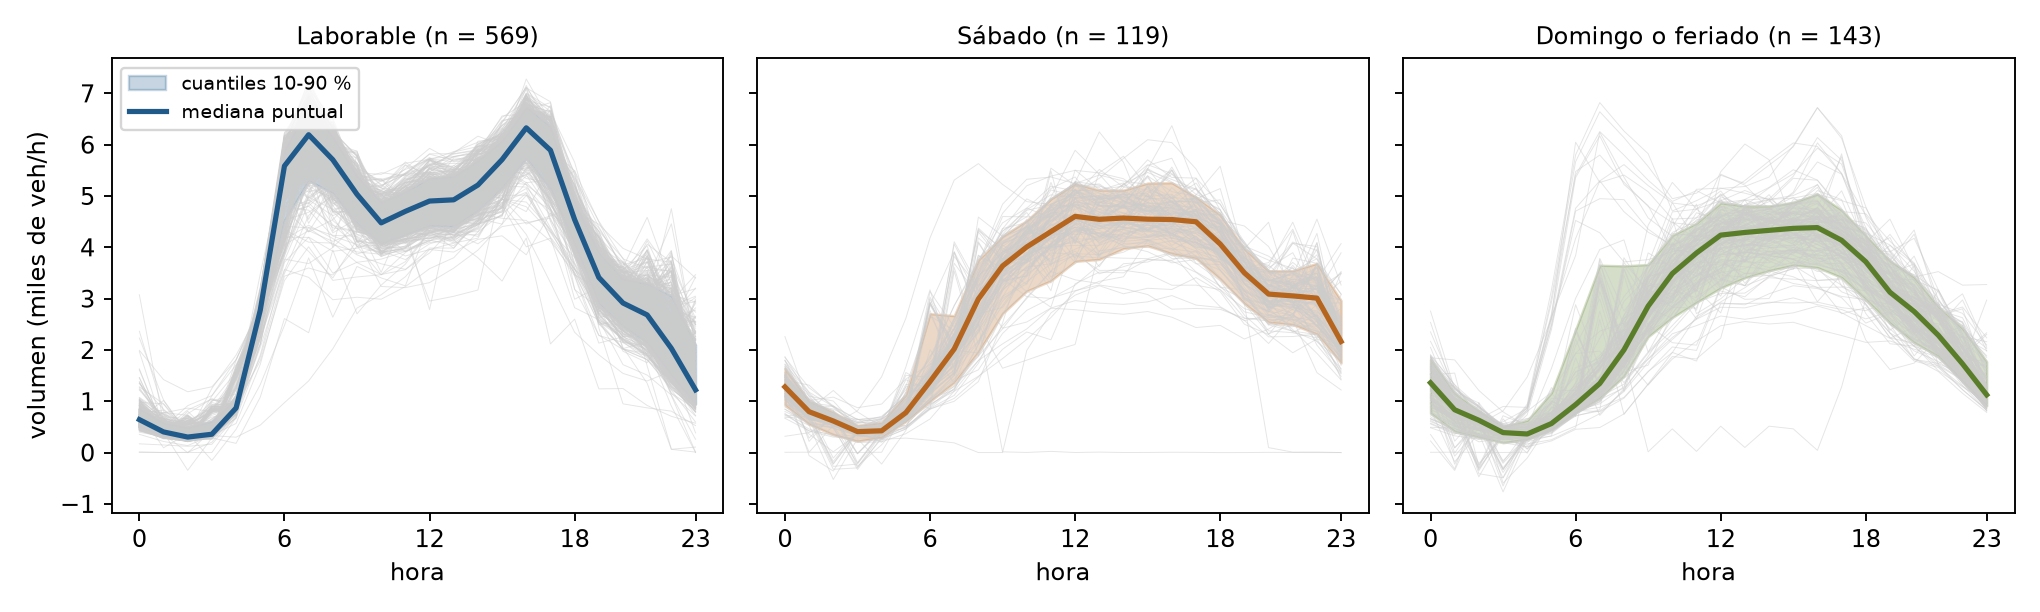
\includegraphics[width=\textwidth,height=0.4\textheight,keepaspectratio]{IMG/04_01/04_perfiles_tipo_dia.png}
\caption{Curvas diarias del bloque de entrenamiento por tipo de día, con la mediana puntual y la banda entre los cuantiles $10\%$ y $90\%$.}
\label{fig:apl_perfiles}
\end{figure}

La Figura~\ref{fig:apl_nivel} muestra el nivel medio de cada día a lo largo de la ventana. Los días laborables forman una franja separada de la de los fines de semana, en la que sábados y domingos quedan próximos entre sí, y ninguna de las franjas tiene tendencia marcada, salvo un nivel laborable algo más bajo en el segundo semestre de 2016. 

\begin{figure}[H]
\centering
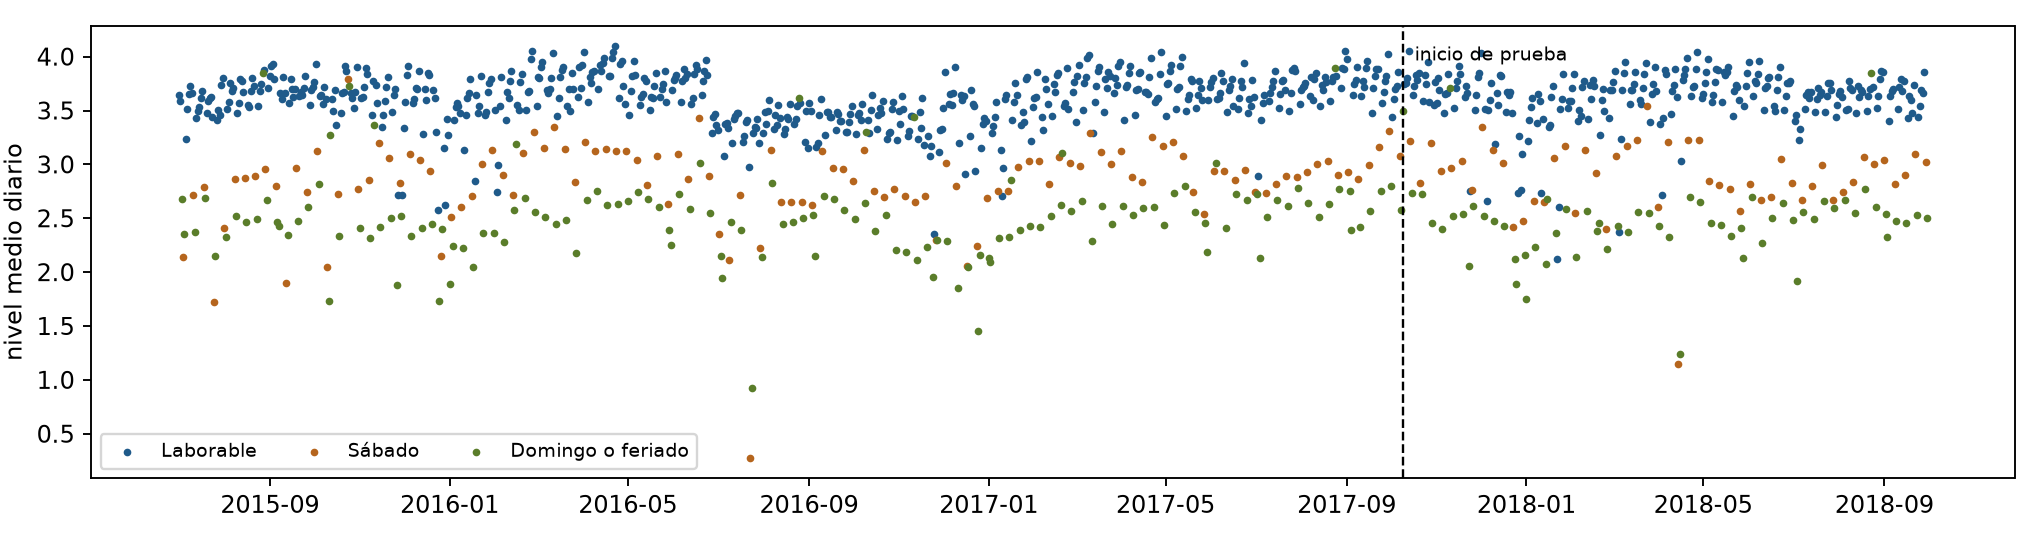
\includegraphics[width=\textwidth,height=0.3\textheight,keepaspectratio]{IMG/04_01/04_nivel_diario.png}
\caption{Nivel medio diario del volumen de tráfico por tipo de día. La línea discontinua marca el inicio del bloque de prueba.}
\label{fig:apl_nivel}
\end{figure}

La Figura~\ref{fig:apl_dependencia} relaciona el primer score, que distingue el perfil laborable del de fin de semana, con su valor un día y una semana antes. Frente al rezago de un día, los puntos forman cuatro nubes, una por cada transición, de laborable a laborable, de viernes a sábado, de sábado a domingo y de domingo a lunes. Un mismo valor del rezago lleva así a destinos distintos, porque tras un día laborable el siguiente puede ser otro laborable o un sábado, y el tercer panel lo muestra de forma directa, pues, condicionado a un rezago en el rango típico de un día laborable, la distribución del score siguiente es bimodal, con un $24\%$ de la masa en el perfil de fin de semana. Una relación lineal con el rezago de un día promedia esos dos destinos en un valor intermedio que no corresponde a ningún día, y por eso explica solo el $16\%$ de la varianza del primer score (correlación $0.40$). Frente al rezago de una semana, en cambio, cada día se compara con el mismo día de la semana anterior, que casi siempre es del mismo tipo, de modo que los puntos se alinean sobre la diagonal y la correlación sube a $0.83$.

\begin{figure}[H]
\centering
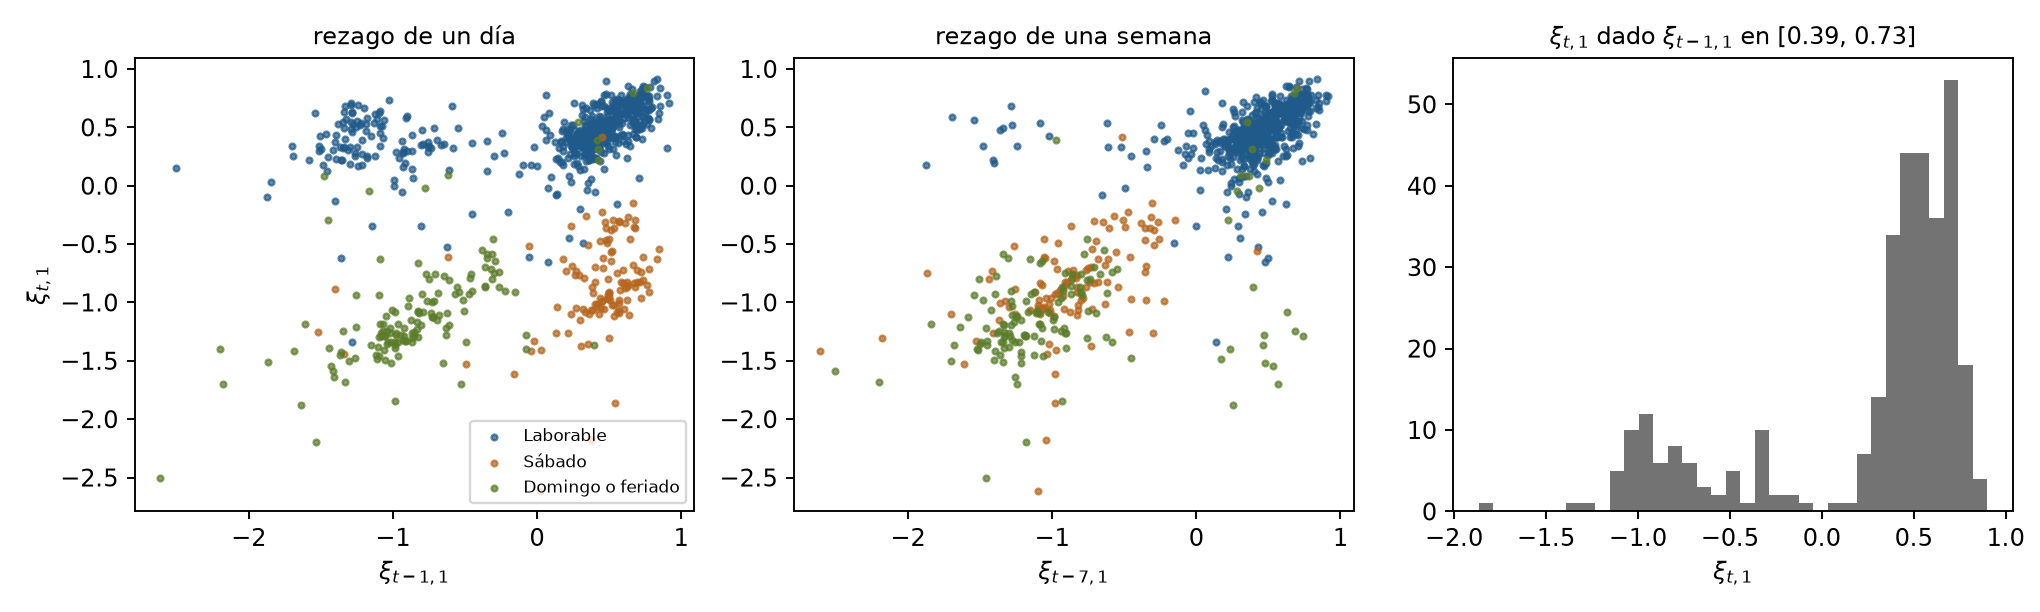
\includegraphics[width=\textwidth,height=0.4\textheight,keepaspectratio]{IMG/04_01/04_dependencia_score1.png}
\caption{Primer score frente a su rezago de un día (izquierda) y de una semana (centro), por tipo de día predicho, y distribución del primer score condicionada a un rezago de un día en el rango típico de los días laborables (derecha). Bloque de entrenamiento.}
\label{fig:apl_dependencia}
\end{figure}

Por tanto, la evidencia descriptiva justifica el uso del modelo propuesto en dos sentidos. Primero, con la información del día anterior la ley de la curva siguiente es una mezcla de perfiles, que un predictor lineal resume en un promedio que no corresponde a ningún día real, mientras que una mezcla con pesos dependientes de las covariables puede asignar un átomo a cada perfil y una probabilidad a cada uno. Segundo, el estado que decide el perfil, el tipo de día, está contenido en buena parte en el rezago semanal, de modo que agregarlo a las covariables de los pesos de la mezcla debería concentrar la masa en el perfil correcto.

\section{Diseño}
\label{04_02_00_diseno}

El diseño sigue al del estudio de simulación (Sección~\ref{03_07_00_diseno_estudio_simulacion}), con las diferencias que impone trabajar con una sola serie observada. Todo lo que se estima con datos, la base, la FPCA, los hiperparámetros del modelo propuesto y los modelos de referencia, se estima solo con el bloque de entrenamiento. Sobre el bloque de prueba se calculan predicciones a un paso con los rezagos observados, sin reestimar ningún modelo, y el calendario no entra a ningún método, se usa solo para leer los resultados.\\

Se ajustan dos especificaciones del PSBPM-FD que difieren en las covariables. En la primera, el score $m$ del día $t$ depende de los diez scores del día $t-1$; en la segunda, de los diez scores de los días $t-1$ y $t-7$, veinte covariables en total. En ambas, cada score tiene su propia mezcla y los pesos de la mezcla dependen de todas las covariables, de modo que la información del rezago semanal puede cambiar los pesos de los átomos sin cambiar su forma. El modelo se ajusta con los hiperparámetros de \citet{03_02_chung2009nonparametric} expresados en la escala de cada score, con $a_\nu = 2$, que a diferencia del valor $0.5$ del estudio de simulación garantiza que la varianza predictiva exista, y con un truncamiento de 30 átomos. El muestreador se ejecuta con una cadena de 2500 iteraciones, de las que se descartan las primeras 1000 como calentamiento; con una sola cadena no se calcula $\widehat{R}$, y los diagnósticos se hacen sobre cantidades invariantes a la permutación de las etiquetas de los átomos.\\

Las referencias son las del estudio de simulación. El FAR se ajusta sobre los coeficientes de la base con orden igual al mayor rezago de cada especificación, uno en la primera y siete en la segunda, y su intervalo es la banda gaussiana de su residuo. El Random Forest ajusta un bosque por score con las mismas covariables que el PSBPM-FD y elige el conjunto de rezagos con el bloque de entrenamiento. Solo el FAR y el PSBPM-FD entregan intervalos.\\

Los resultados se presentan como en la Sección~\ref{03_08_00_resultados}. Las métricas de la Sección~\ref{02_02_03_criterios_evaluacion} se calculan sobre la ventana móvil de ancho $w = 30$ sobre el bloque de prueba, contra la curva ajustada por la representación (Sección~\ref{03_05_00_reconstruccion_funcional}), y los cuadros reportan su promedio sobre las ventanas y la fracción de ventanas que gana cada modelo. Del PSBPM-FD se reportan los tres predictores puntuales de la Sección~\ref{03_05_04_predictores_puntuales}, con la regla de consistencia según la cual el MAE corresponde a la mediana puntual y el RMSE a la esperanza, y las tres construcciones de intervalo de la Sección~\ref{03_05_05_intervalos_predictivos}. Los comportamientos predictivos (Sección~\ref{03_06_00_comportamientos}) se resumen por la distribución de $K_t$ en el bloque de prueba y se contrastan con el calendario, que aquí reemplaza al régimen verdadero de la simulación. Para mostrar qué es un comportamiento se analiza una ventana de detalle de diez días consecutivos de prueba, elegida por tener la mayor cantidad de días no laborables, del 23 de diciembre de 2017 al 1 de enero de 2018, con dos fines de semana, Navidad y Año Nuevo. Se evalúa además el pronóstico por comportamiento de la Sección~\ref{03_06_03_descripcion} y su cota \eqref{eq:mejor_comportamiento}, y, por último, se analizan las probabilidades posteriores de inclusión de los rezagos en la mezcla de cada score. La configuración completa de la aplicación está en el Anexo~\ref{aneC_00_01_configuracion}.

Los resultados siguen el orden del estudio de simulación, es decir, error puntual, intervalos de predicción, comportamientos predictivos y el pronóstico que se construye con ellos, y se agrega al final la selección de variables. En cada apartado se contrastan las dos especificaciones, porque la diferencia entre ellas es la que muestra el efecto de la información sobre los pesos de la mezcla.

\subsection{Error puntual}
\label{04_03_01_error_puntual}

Los Cuadros~\ref{tab:apl_bloqueA} y~\ref{tab:apl_bloqueA_ganancia} resumen el MAE y el RMSE promedio sobre las ventanas de prueba de los tres predictores del PSBPM-FD y de las dos referencias, y el cambio relativo respecto del FAR.

% Fuente: 98_resumen_bloqueA_min_max_prom.csv del _05 (test, promedio sobre ventanas).
\begin{table}[H]
\centering\small
\setlength{\tabcolsep}{3.5pt}
\caption{MAE y RMSE en el bloque de prueba del tráfico ($M = 10$, $w = 30$). En negrita el menor de cada fila.}
\label{tab:apl_bloqueA}
\begin{tabular}{l ccccc ccccc}
\hline
Rezagos & \multicolumn{5}{c}{MAE} & \multicolumn{5}{c}{RMSE} \\
 & Esp. & Med. & Modal & RF & FAR & Esp. & Med. & Modal & RF & FAR \\
\hline
$\{1\}$ & 0.413 & 0.376 & 0.397 & \textbf{0.361} & 0.398 & 0.646 & 0.658 & 0.729 & \textbf{0.562} & 0.621 \\
$\{1,7\}$ & 0.315 & \textbf{0.302} & 0.317 & 0.314 & 0.314 & 0.522 & 0.528 & 0.556 & 0.499 & \textbf{0.495} \\
\hline
\end{tabular}
\end{table}

\begin{table}[H]
\centering\small
\setlength{\tabcolsep}{3.5pt}
\caption{Cambio relativo del MAE y del RMSE respecto del FAR por predictor. Negativo es mejor que el FAR.}
\label{tab:apl_bloqueA_ganancia}
\begin{tabular}{l cc cc cc cc}
\hline
Rezagos & \multicolumn{2}{c}{Esperanza} & \multicolumn{2}{c}{Mediana} & \multicolumn{2}{c}{Modal} & \multicolumn{2}{c}{RF} \\
 & MAE & RMSE & MAE & RMSE & MAE & RMSE & MAE & RMSE \\
\hline
$\{1\}$ & $+3.8\%$ & $+4.1\%$ & $-5.4\%$ & $+5.9\%$ & $-0.1\%$ & $+17.4\%$ & $-9.3\%$ & $-9.6\%$ \\
$\{1,7\}$ & $+0.1\%$ & $+5.6\%$ & $-3.7\%$ & $+6.6\%$ & $+1.0\%$ & $+12.3\%$ & $0.0\%$ & $+0.8\%$ \\
\hline
\end{tabular}
\end{table}
Al agregar el rezago semanal, el MAE de todos los modelos baja entre un $13\%$ y un $24\%$, y el FAR con ambos rezagos ($0.314$) queda por debajo de cualquier modelo con solo el rezago de un día, incluido el Random Forest ($0.361$). Además, la comparación entre los predictores del PSBPM-FD reproduce lo que anticipa la forma de la predictiva. Con el rezago de un día, donde la predictiva tiene dos comportamientos en la mayoría de los orígenes (Sección~\ref{04_03_03_comportamientos}), la esperanza queda entre el perfil laborable y el de fin de semana, en una curva que no ocurre, y pierde frente al FAR en las dos métricas. La mediana puntual se inclina hacia el comportamiento dominante y baja el MAE del FAR en un $5.4\%$, pero cuando el comportamiento dominante no es el que ocurre su error es grande y su RMSE sube, que es el reparto que corresponde a lo que mide cada métrica. El átomo más probable es el peor en RMSE en las dos especificaciones. Con ambos rezagos, la mediana sigue siendo la mejor en MAE ($-3.7\%$) y la esperanza, el FAR y el Random Forest quedan a menos de un $1\%$ entre sí, mientras que en RMSE el FAR es el mejor.\\

El Random Forest es el mejor modelo con el rezago de un día, por un margen de un $9\%$ sobre el FAR en las dos métricas, y su ventaja desaparece con el rezago semanal. Con una sola covariable diaria, la partición por umbrales del bosque separa los destinos posibles de un día laborable mejor que un promedio, y cuando el rezago semanal resuelve el tipo de día la parte lineal de la dinámica basta y las diferencias entre métodos desaparecen.

% Fuente: 72_ventana_modelos_w30.csv del _05 (test, w = 30, sin el medoide).
\begin{table}[H]
\centering\small
\setlength{\tabcolsep}{3.5pt}
\caption{Ventanas de prueba ganadas por modelo, por MAE y por RMSE.}
\label{tab:apl_bloqueA_ventanas}
\begin{tabular}{l ccccc ccccc}
\hline
Rezagos & \multicolumn{5}{c}{MAE} & \multicolumn{5}{c}{RMSE} \\
 & FAR & RF & Esp. & Med. & Modal & FAR & RF & Esp. & Med. & Modal \\
\hline
$\{1\}$ & 7\% & 54\% & 0\% & 25\% & 14\% & 11\% & 78\% & 0\% & 9\% & 1\% \\
$\{1,7\}$ & 18\% & 19\% & 1\% & 59\% & 3\% & 43\% & 37\% & 1\% & 19\% & 0\% \\
\hline
\end{tabular}
\end{table}

\begin{table}[H]
\centering\small
\setlength{\tabcolsep}{3.5pt}
\caption{Fracción de ventanas en que el predictor consistente del PSBPM-FD supera a cada referencia (mediana en MAE, esperanza en RMSE).}
\label{tab:apl_bloqueA_gana}
\begin{tabular}{l cc cc}
\hline
Rezagos & \multicolumn{2}{c}{MAE (mediana)} & \multicolumn{2}{c}{RMSE (esperanza)} \\
 & vs FAR & vs RF & vs FAR & vs RF \\
\hline
$\{1\}$ & 70\% & 42\% & 27\% & 1\% \\
$\{1,7\}$ & 80\% & 73\% & 21\% & 30\% \\
\hline
\end{tabular}
\end{table}

Los Cuadros~\ref{tab:apl_bloqueA_ventanas} y~\ref{tab:apl_bloqueA_gana} muestran que los promedios se sostienen a lo largo del bloque de prueba. Bajo MAE, la mediana puntual supera al FAR en siete de cada diez ventanas con el rezago de un día y en ocho de cada diez con ambos rezagos, y con ambos rezagos es el mejor modelo en el $59\%$ de las ventanas y supera al Random Forest en el $73\%$. Bajo RMSE la ventaja es de las referencias, ya que la esperanza supera al FAR en menos de un tercio de las ventanas en las dos especificaciones, y con el rezago de un día el Random Forest gana el $78\%$ de ellas.

% Fuente: 72_ventana_modelos_w30.csv de 101 y 102 (test, sin el medoide); figura en docs/IMG/04_03.
\begin{figure}[H]
\centering
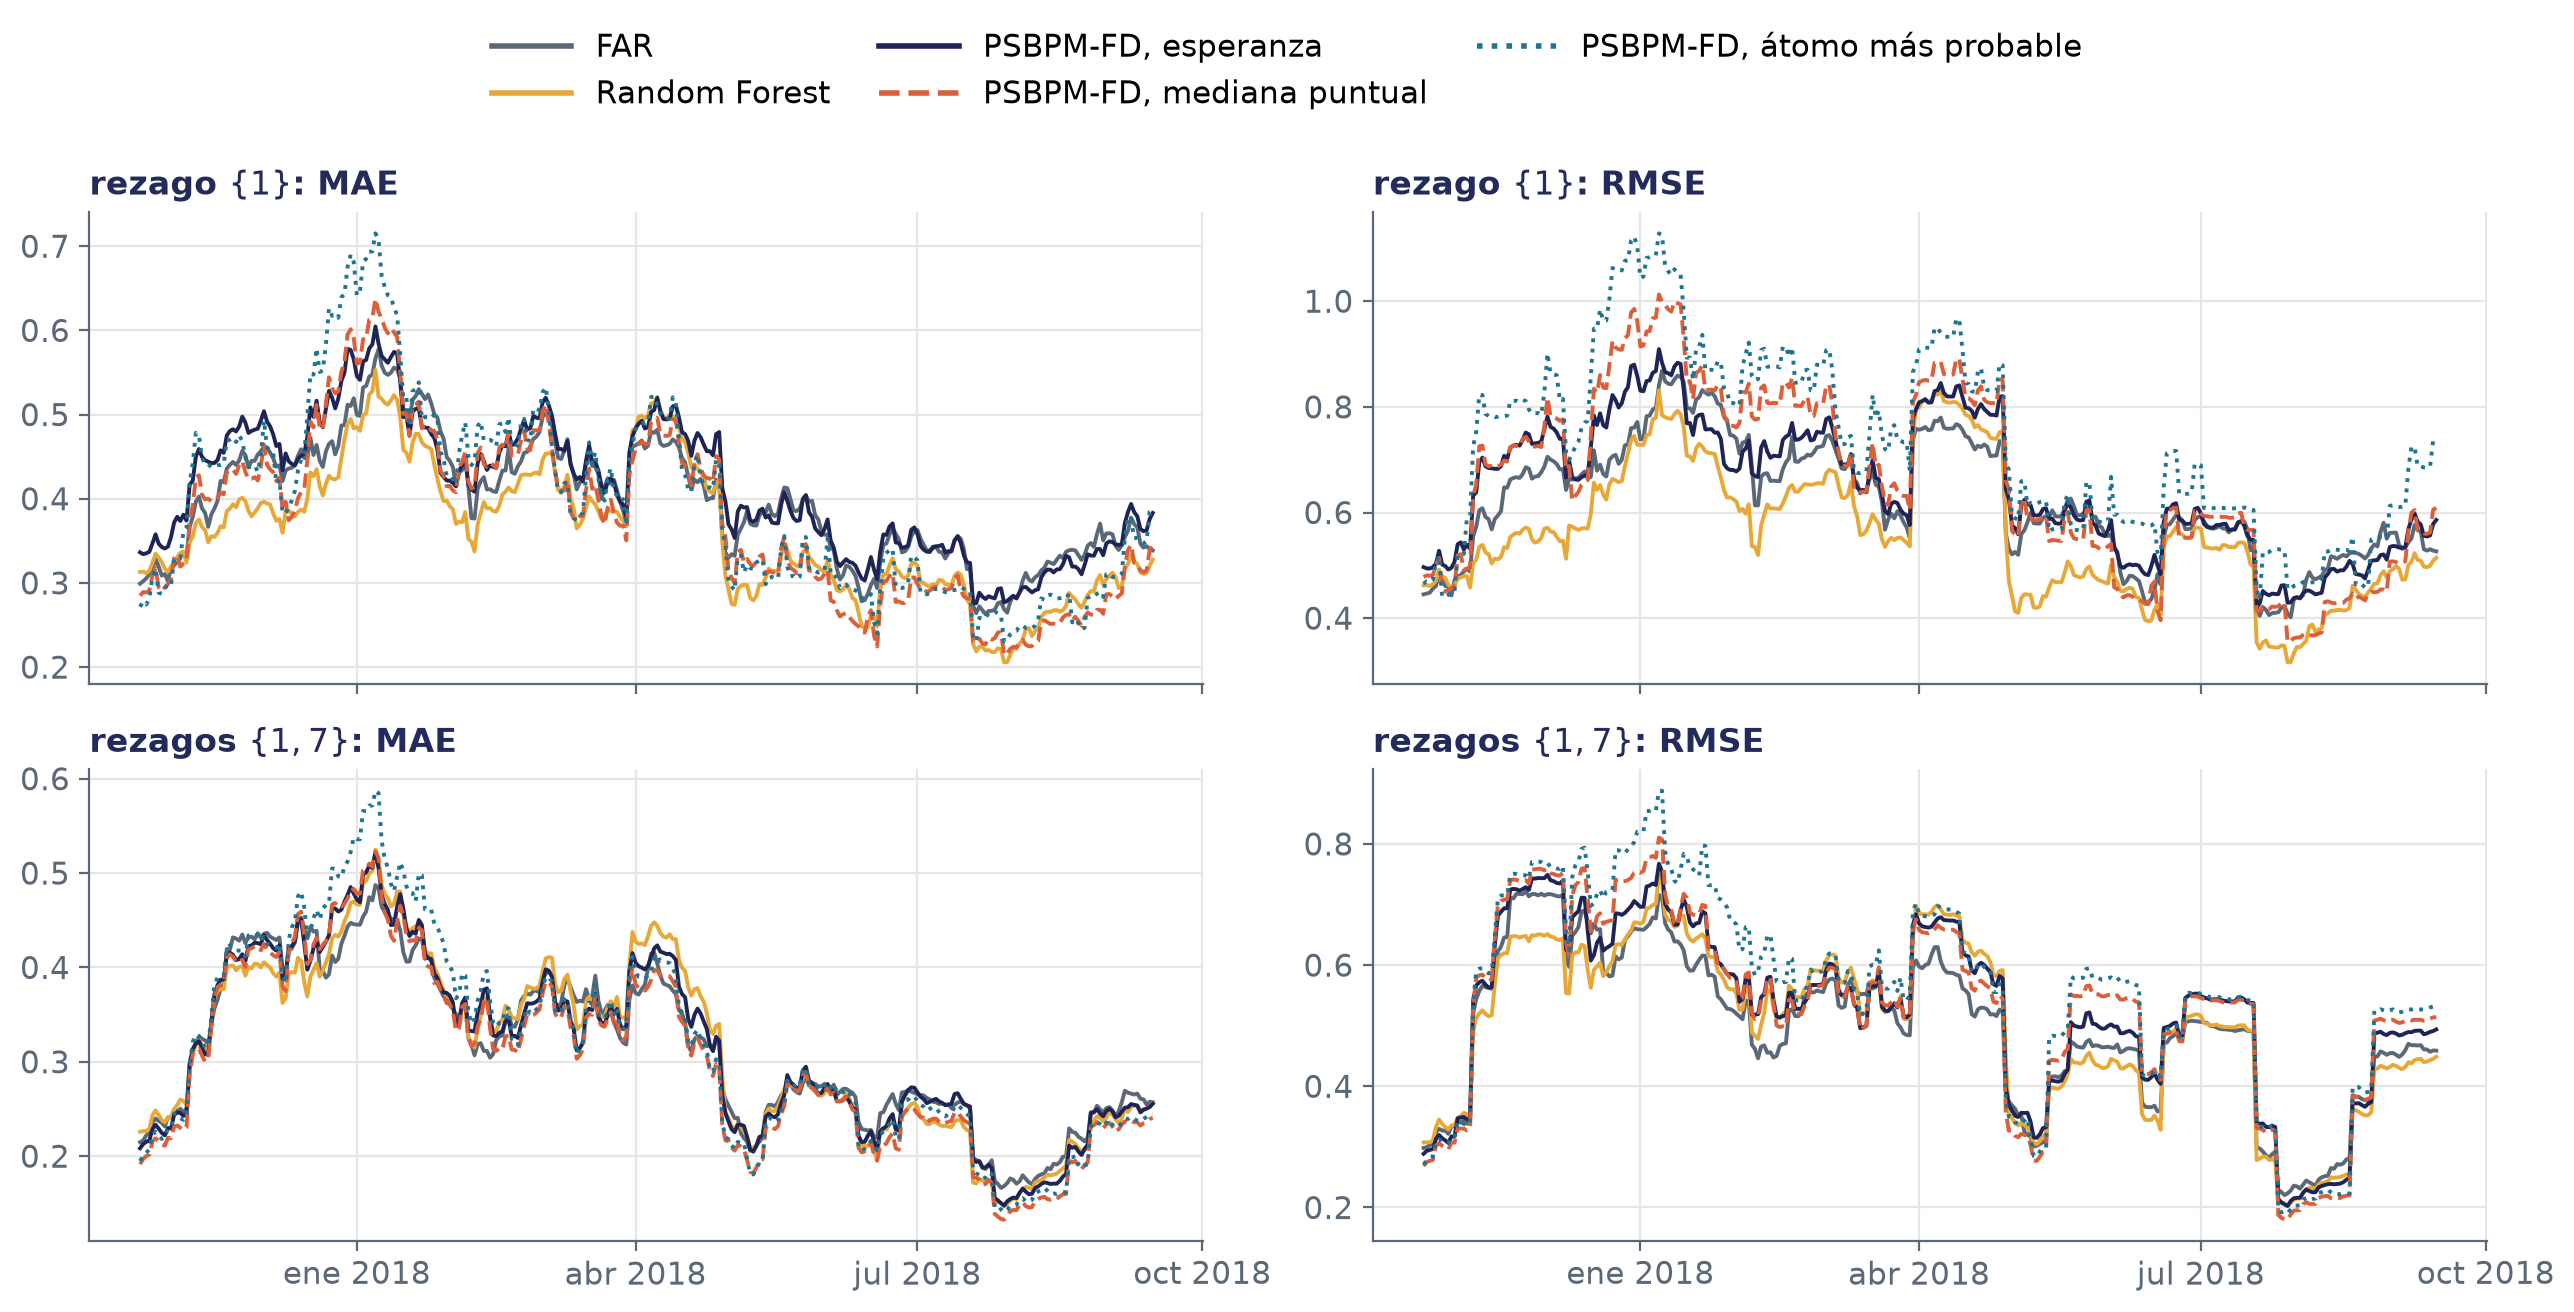
\includegraphics[width=\textwidth]{IMG/04_03/04_bloqueA_ventana_w30.png}
\caption{MAE y RMSE sobre la ventana móvil del bloque de prueba, con rezago $\{1\}$ (arriba) y rezagos $\{1,7\}$ (abajo) ($M = 10$, $w = 30$).}
\label{fig:apl_bloqueA_ventana}
\end{figure}

La Figura~\ref{fig:apl_bloqueA_ventana} muestra que todos los modelos suben y bajan juntos, y el máximo se alcanza en las ventanas que contienen el período de fiestas de fin de año, donde se concentran los feriados que ningún rezago anuncia. Con el rezago de un día las curvas se separan, el Random Forest queda debajo en buena parte del bloque y el átomo más probable se despega hacia arriba en RMSE en los meses de invierno; con ambos rezagos las curvas de todos los modelos casi se superponen, que es la imagen en el tiempo de lo que muestran los cuadros, es decir, la información sobre el tipo de día elimina las diferencias entre métodos en el error puntual.

\subsection{Intervalos de predicción}
\label{04_03_02_intervalos}

Los Cuadros~\ref{tab:apl_bloqueB_winkler} y~\ref{tab:apl_bloqueB_picp} resumen el Winkler, el MPIW, el PICP y el PICPB de las tres construcciones del PSBPM-FD y de la banda gaussiana del FAR, al nivel nominal de $95\%$.

% Fuente: 99_resumen_bloqueB_min_max_prom.csv y 81_ventana_bloqueB_w30.csv del _05.
\begin{table}[H]
\centering\small
\setlength{\tabcolsep}{3.5pt}
\caption{Winkler y MPIW en el bloque de prueba del tráfico ($M = 10$). En negrita el menor Winkler de cada fila.}
\label{tab:apl_bloqueB_winkler}
\begin{tabular}{l cccc cccc}
\hline
Rezagos & \multicolumn{4}{c}{Winkler} & \multicolumn{4}{c}{MPIW} \\
 & FAR & Equi. & HDR & Simult. & FAR & Equi. & HDR & Simult. \\
\hline
$\{1\}$ & 3.073 & 2.734 & \textbf{2.669} & 4.493 & 2.159 & 2.124 & 1.995 & 4.242 \\
$\{1,7\}$ & 3.052 & \textbf{2.707} & 2.714 & 3.549 & 1.602 & 1.752 & 1.689 & 3.011 \\
\hline
\end{tabular}
\end{table}

\begin{table}[H]
\centering\small
\setlength{\tabcolsep}{3.5pt}
\caption{PICP y PICPB en el bloque de prueba del tráfico ($M = 10$). Nominal $0.95$.}
\label{tab:apl_bloqueB_picp}
\begin{tabular}{l cccc cccc}
\hline
Rezagos & \multicolumn{4}{c}{PICP} & \multicolumn{4}{c}{PICPB} \\
 & FAR & Equi. & HDR & Simult. & FAR & Equi. & HDR & Simult. \\
\hline
$\{1\}$ & 0.950 & 0.961 & 0.960 & 0.991 & 0.721 & 0.731 & 0.742 & 0.942 \\
$\{1,7\}$ & 0.930 & 0.956 & 0.955 & 0.983 & 0.675 & 0.754 & 0.746 & 0.917 \\
\hline
\end{tabular}
\end{table}

En los intervalos el PSBPM-FD supera al FAR en las dos especificaciones. Las bandas puntuales, equi-colas y de máxima densidad, bajan el Winkler del FAR en un $11\%$ a $13\%$ y cubren el $96\%$ del dominio, por sobre el $93\%$ a $95\%$ del FAR. La ganancia no depende del rezago semanal, a diferencia del error puntual, ya que aun cuando la información resuelve el tipo de día, la incertidumbre alrededor del perfil sigue cambiando de un origen a otro, y una banda de ancho fijo no puede seguirla. Ninguna banda puntual cubre la curva completa con la frecuencia nominal, porque su PICPB queda entre $0.68$ y $0.75$; la simultánea, la única construida para esa cobertura, la alcanza casi ($0.92$ a $0.94$) al precio de casi duplicar el ancho, y por eso pierde el Winkler.

\begin{table}[H]
\centering\small
\setlength{\tabcolsep}{3pt}
\caption{Cambio relativo del Winkler y del MPIW respecto del FAR por construcción. Negativo es mejor que el FAR.}
\label{tab:apl_bloqueB_ganancia}
\begin{tabular}{l cc cc cc}
\hline
Rezagos & \multicolumn{2}{c}{Equi-colas} & \multicolumn{2}{c}{Máxima densidad} & \multicolumn{2}{c}{Simultánea} \\
 & Winkler & MPIW & Winkler & MPIW & Winkler & MPIW \\
\hline
$\{1\}$ & $-11.0\%$ & $-1.6\%$ & $-13.2\%$ & $-7.6\%$ & $+46.2\%$ & $+96.5\%$ \\
$\{1,7\}$ & $-11.3\%$ & $+9.4\%$ & $-11.1\%$ & $+5.4\%$ & $+16.3\%$ & $+88.0\%$ \\
\hline
\end{tabular}
\end{table}

El Cuadro~\ref{tab:apl_bloqueB_ganancia} muestra que la composición de la ganancia cambia con la información. Con el rezago de un día las bandas del PSBPM-FD son más angostas que la del FAR y además cubren más, y la de máxima densidad es la más angosta de todas ($-7.6\%$), porque cuando la predictiva tiene dos comportamientos reparte su masa entre ellos en lugar de gastarla en el valle intermedio, como hace la equi-colas. Con ambos rezagos las bandas son un $5\%$ a $9\%$ más anchas que la del FAR y ganan por cobertura, porque la del FAR, al estrecharse con la mejor información, queda corta ($0.93$ de PICP) en los días que el rezago semanal no anuncia. La máxima densidad coincide entonces con la equi-colas, como en los escenarios unimodales de la simulación.

% Fuente: 81_ventana_bloqueB_w30.csv (test, w = 30).
\begin{table}[H]
\centering\small
\setlength{\tabcolsep}{3.5pt}
\caption{Ventanas de prueba ganadas por Winkler.}
\label{tab:apl_bloqueB_ventanas}
\begin{tabular}{l cccc ccc}
\hline
Rezagos & \multicolumn{4}{c}{La mejor banda} & \multicolumn{3}{c}{Gana al FAR} \\
 & FAR & Equi. & HDR & Simult. & Equi. & HDR & Simult. \\
\hline
$\{1\}$ & 3\% & 21\% & 76\% & 0\% & 93\% & 93\% & 4\% \\
$\{1,7\}$ & 22\% & 26\% & 52\% & 0\% & 76\% & 75\% & 12\% \\
\hline
\end{tabular}
\end{table}

Las bandas puntuales superan al FAR en el $93\%$ de las ventanas con el rezago de un día y en tres de cada cuatro con ambos rezagos (Cuadro~\ref{tab:apl_bloqueB_ventanas}), y la de máxima densidad es la mejor de todas en el $76\%$ y el $52\%$ de ellas. La simultánea no es la mejor en ninguna ventana.

% Fuente: 81_ventana_bloqueB_w30.csv de 101 y 102 (test); figura en docs/IMG/04_03.
\begin{figure}[H]
\centering
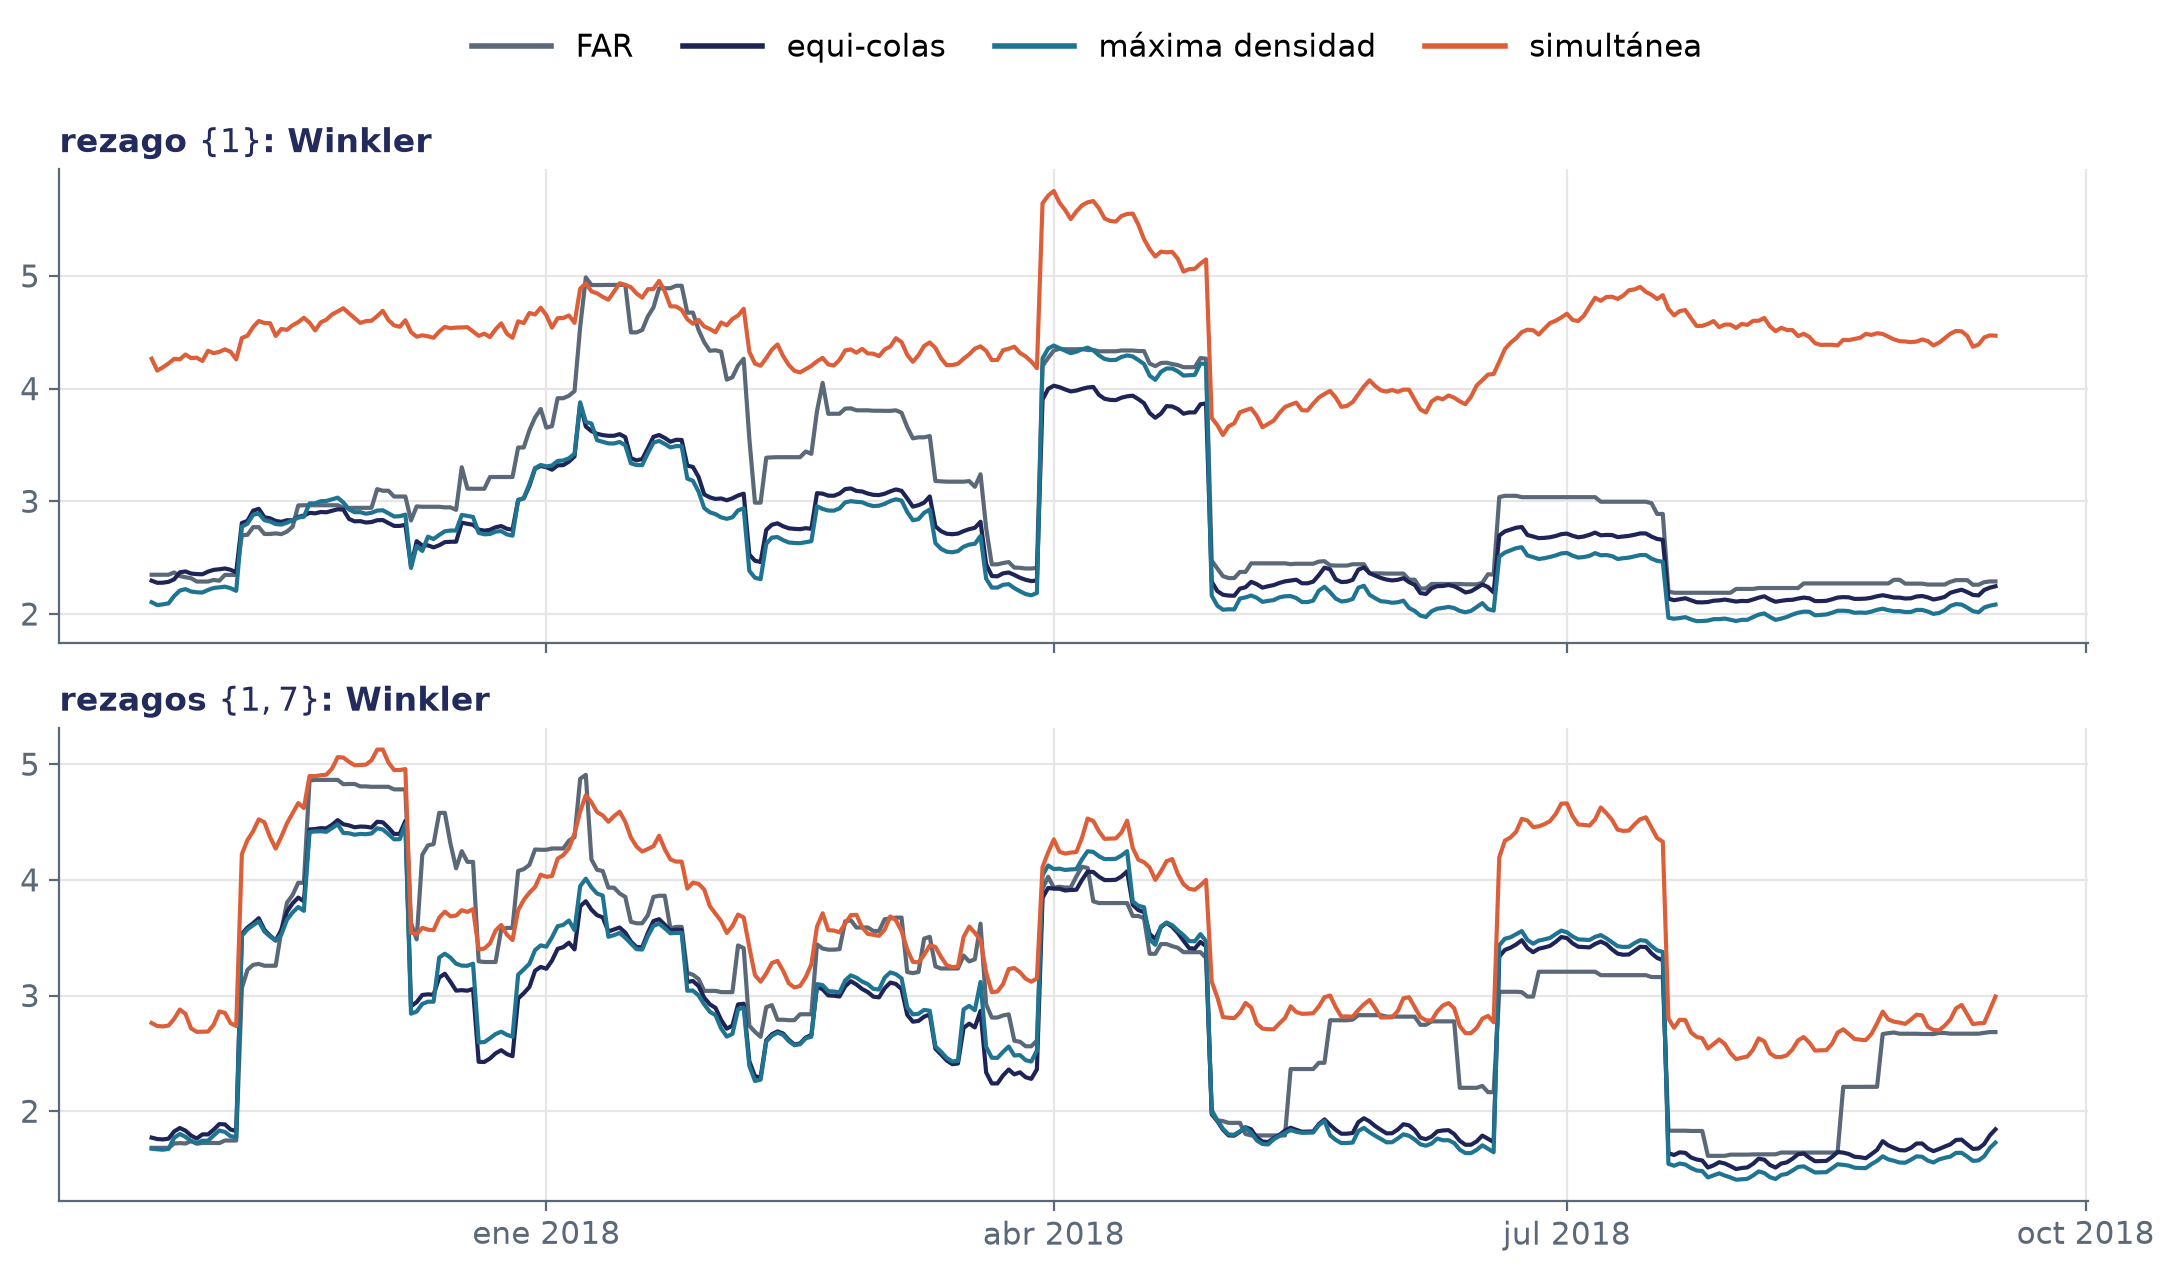
\includegraphics[width=\textwidth]{IMG/04_03/04_bloqueB_ventana_w30.png}
\caption{Winkler sobre la ventana móvil del bloque de prueba, con rezago $\{1\}$ (arriba) y rezagos $\{1,7\}$ (abajo) ($M = 10$, $w = 30$).}
\label{fig:apl_bloqueB_ventana}
\end{figure}

La Figura~\ref{fig:apl_bloqueB_ventana} muestra el Winkler a lo largo del bloque de prueba. En las dos especificaciones las bandas puntuales del PSBPM-FD quedan bajo el FAR en la mayor parte de las ventanas, y la diferencia es mayor en las del invierno, que incluyen el período de fiestas de fin de año, donde el Winkler del FAR aumenta por los días que su banda no cubre. Con ambos rezagos hay tramos, en abril y en julio, en que la banda del PSBPM-FD queda por encima del FAR, y son los que bajan su fracción de ventanas ganadas al $76\%$.\\

% Fuente: banda_funcional_psbp.npz del _04 (li, ls, hdr_L, hdr_U, li/ls_simultanea) y MPIW del FAR de 81_*.
\begin{figure}[H]
\centering
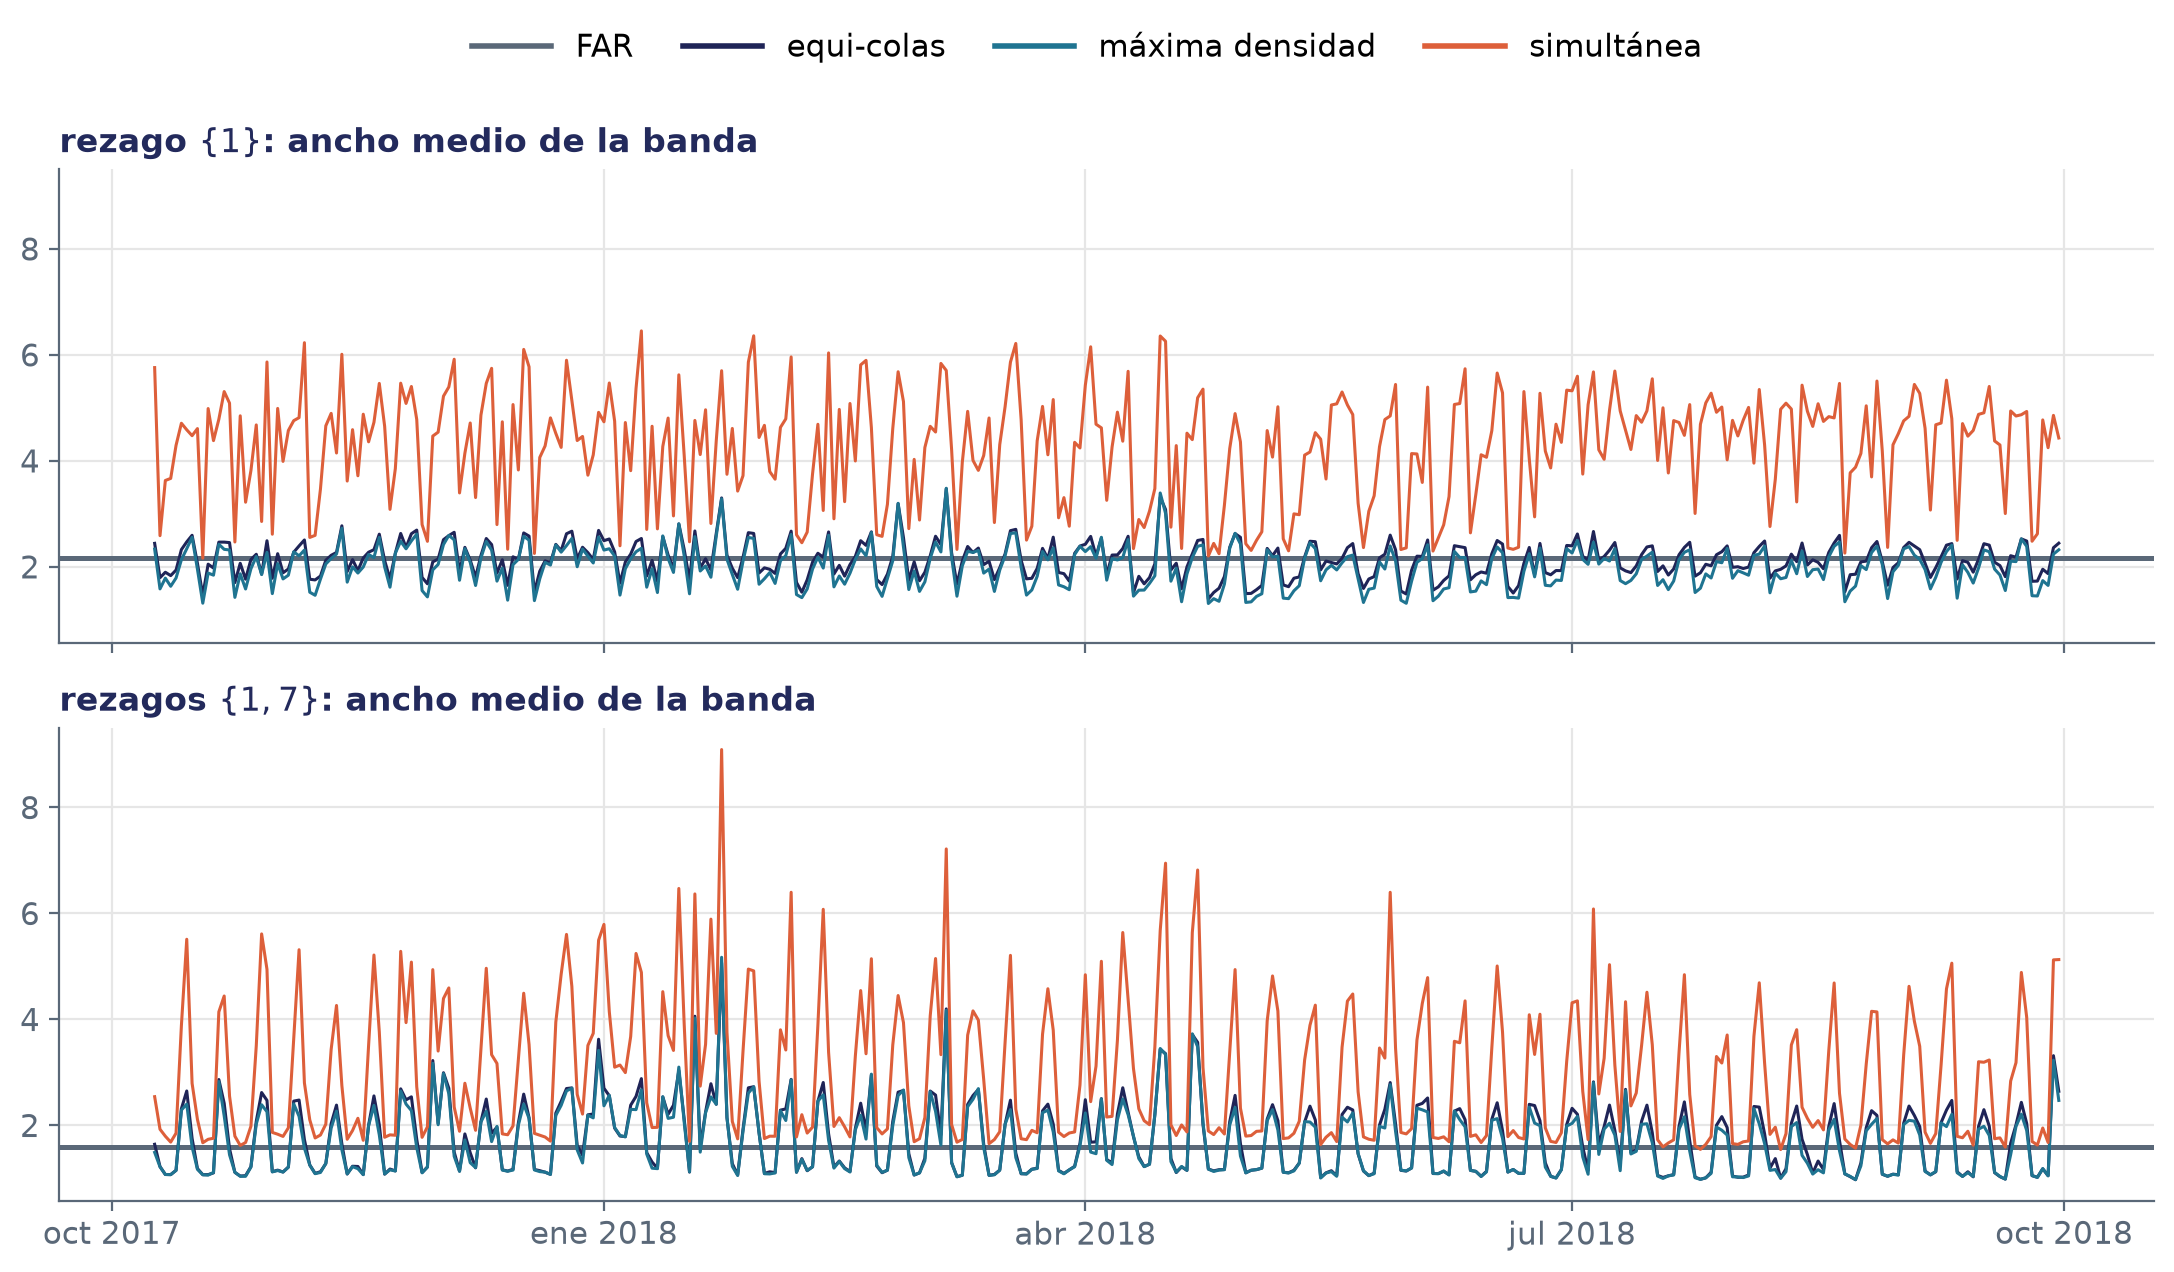
\includegraphics[width=\textwidth]{IMG/04_03/04_bloqueB_ancho.png}
\caption{Ancho medio de la banda en cada origen de prueba de las tres construcciones del PSBPM-FD y ancho fijo del FAR, con rezago $\{1\}$ (arriba) y rezagos $\{1,7\}$ (abajo) ($M = 10$).}
\label{fig:apl_bloqueB_ancho}
\end{figure}

La Figura~\ref{fig:apl_bloqueB_ancho} muestra que el ancho de la banda del FAR es el mismo en todos los orígenes, mientras que el del PSBPM-FD cambia con el tipo de día. Con ambos rezagos la banda equi-colas es más angosta que la del FAR en el $71\%$ de los días laborables, con un ancho medio de $1.48$ frente a $1.60$, y más ancha en el $96\%$ de los no laborables, con $2.34$, que son los días en que el rezago semanal ya no decide el perfil. Con el rezago de un día el patrón es menos marcado ($2.06$ en los laborables y $2.34$ en los no laborables, frente a $2.16$ del FAR), porque la predictiva ya reparte su masa entre los dos perfiles en la mayoría de los días.

\subsection{Comportamientos predictivos}
\label{04_03_03_comportamientos}

El Cuadro~\ref{tab:apl_K} resume cuántos comportamientos declara el modelo en el bloque de prueba con cada especificación.

% Fuente: 102_K_por_M.csv del barrido (bloque test, M = 10).
\begin{table}[H]
\centering\small
\setlength{\tabcolsep}{3.5pt}
\caption{Distribución de $K_t$ en el bloque de prueba del tráfico ($M = 10$).}
\label{tab:apl_K}
\begin{tabular}{l c ccc}
\hline
Rezagos & Orígenes & $K_t = 1$ & $K_t = 2$ & $K_t \ge 3$ \\
\hline
$\{1\}$ & 357 & 28.3\% & 71.7\% & 0.0\% \\
$\{1,7\}$ & 357 & 64.1\% & 35.0\% & 0.8\% \\
\hline
\end{tabular}
\end{table}

Con el rezago de un día el modelo declara dos comportamientos en el $72\%$ de los orígenes de prueba, y con ambos rezagos esa fracción baja a la mitad. A diferencia de la simulación, aquí no hay un régimen verdadero con el que contrastar los comportamientos, pero el calendario lo reemplaza, porque el tipo de día es el estado que decide el perfil y no entra al modelo. El Cuadro~\ref{tab:apl_K_calendario} cruza la presencia de más de un comportamiento con el día predicho.

% Fuente: 65_comportamientos_calendario.csv de 101 y 102 (test, 357 orígenes; 51 por día de la semana).
\begin{table}[H]
\centering\small
\caption{Fracción de orígenes de prueba con más de un comportamiento ($K_t \ge 2$) según el día predicho, con y sin el rezago de una semana ($M = 10$).}
\label{tab:apl_K_calendario}
\begin{tabular}{l c cc}
\hline
Día predicho & Orígenes & $\{1\}$ & $\{1,7\}$ \\
\hline
Lunes     & 51  & 100\% & 49\% \\
Martes    & 51  & 41\%  & 12\% \\
Miércoles & 51  & 57\%  & 4\%  \\
Jueves    & 51  & 49\%  & 6\%  \\
Viernes   & 51  & 75\%  & 8\%  \\
Sábado    & 51  & 94\%  & 90\% \\
Domingo   & 51  & 86\%  & 82\% \\
\hline
Laborables    & 244 & 64\% & 14\% \\
No laborables (fin de semana y feriados) & 113 & 89\% & 82\% \\
\hline
\end{tabular}
\end{table}

 Con el rezago de un día hay más de un comportamiento en todos los días de la semana, y sobre todo los lunes y los sábados, los días en que el perfil cambia respecto del anterior, ya que la curva del domingo no distingue un lunes laborable de un lunes feriado, y la del viernes no anuncia el cambio al fin de semana con la claridad suficiente para que la mezcla excluya el perfil laborable. Con ambos rezagos los comportamientos desaparecen de martes a viernes, donde quedan entre un $4\%$ y un $12\%$ de los orígenes, porque la curva de la semana anterior fija el perfil, y la predictiva se vuelve unimodal. Se mantienen en los días no laborables y la mitad de los lunes, que son los días en que el rezago semanal no basta, porque los feriados caen en días que la semana anterior fueron laborables, y los fines de semana tienen una variabilidad propia, de salidas y eventos, que ningún rezago resuelve. De los 256 orígenes con más de un comportamiento en la primera especificación, 139 pasan a tener uno solo en la segunda, mientras que solo 11 hacen el camino inverso. La mezcla no genera comportamientos donde la información alcanza para decidir el perfil, y los conserva donde no alcanza, que es lo que se espera de pesos que dependen de las covariables.

% Fuente: comportamientos_psbp.npz y banda_funcional_psbp.npz del _04 de 101 y 102, curva suavizada (theta @ phi^T).
\begin{figure}[H]
\centering
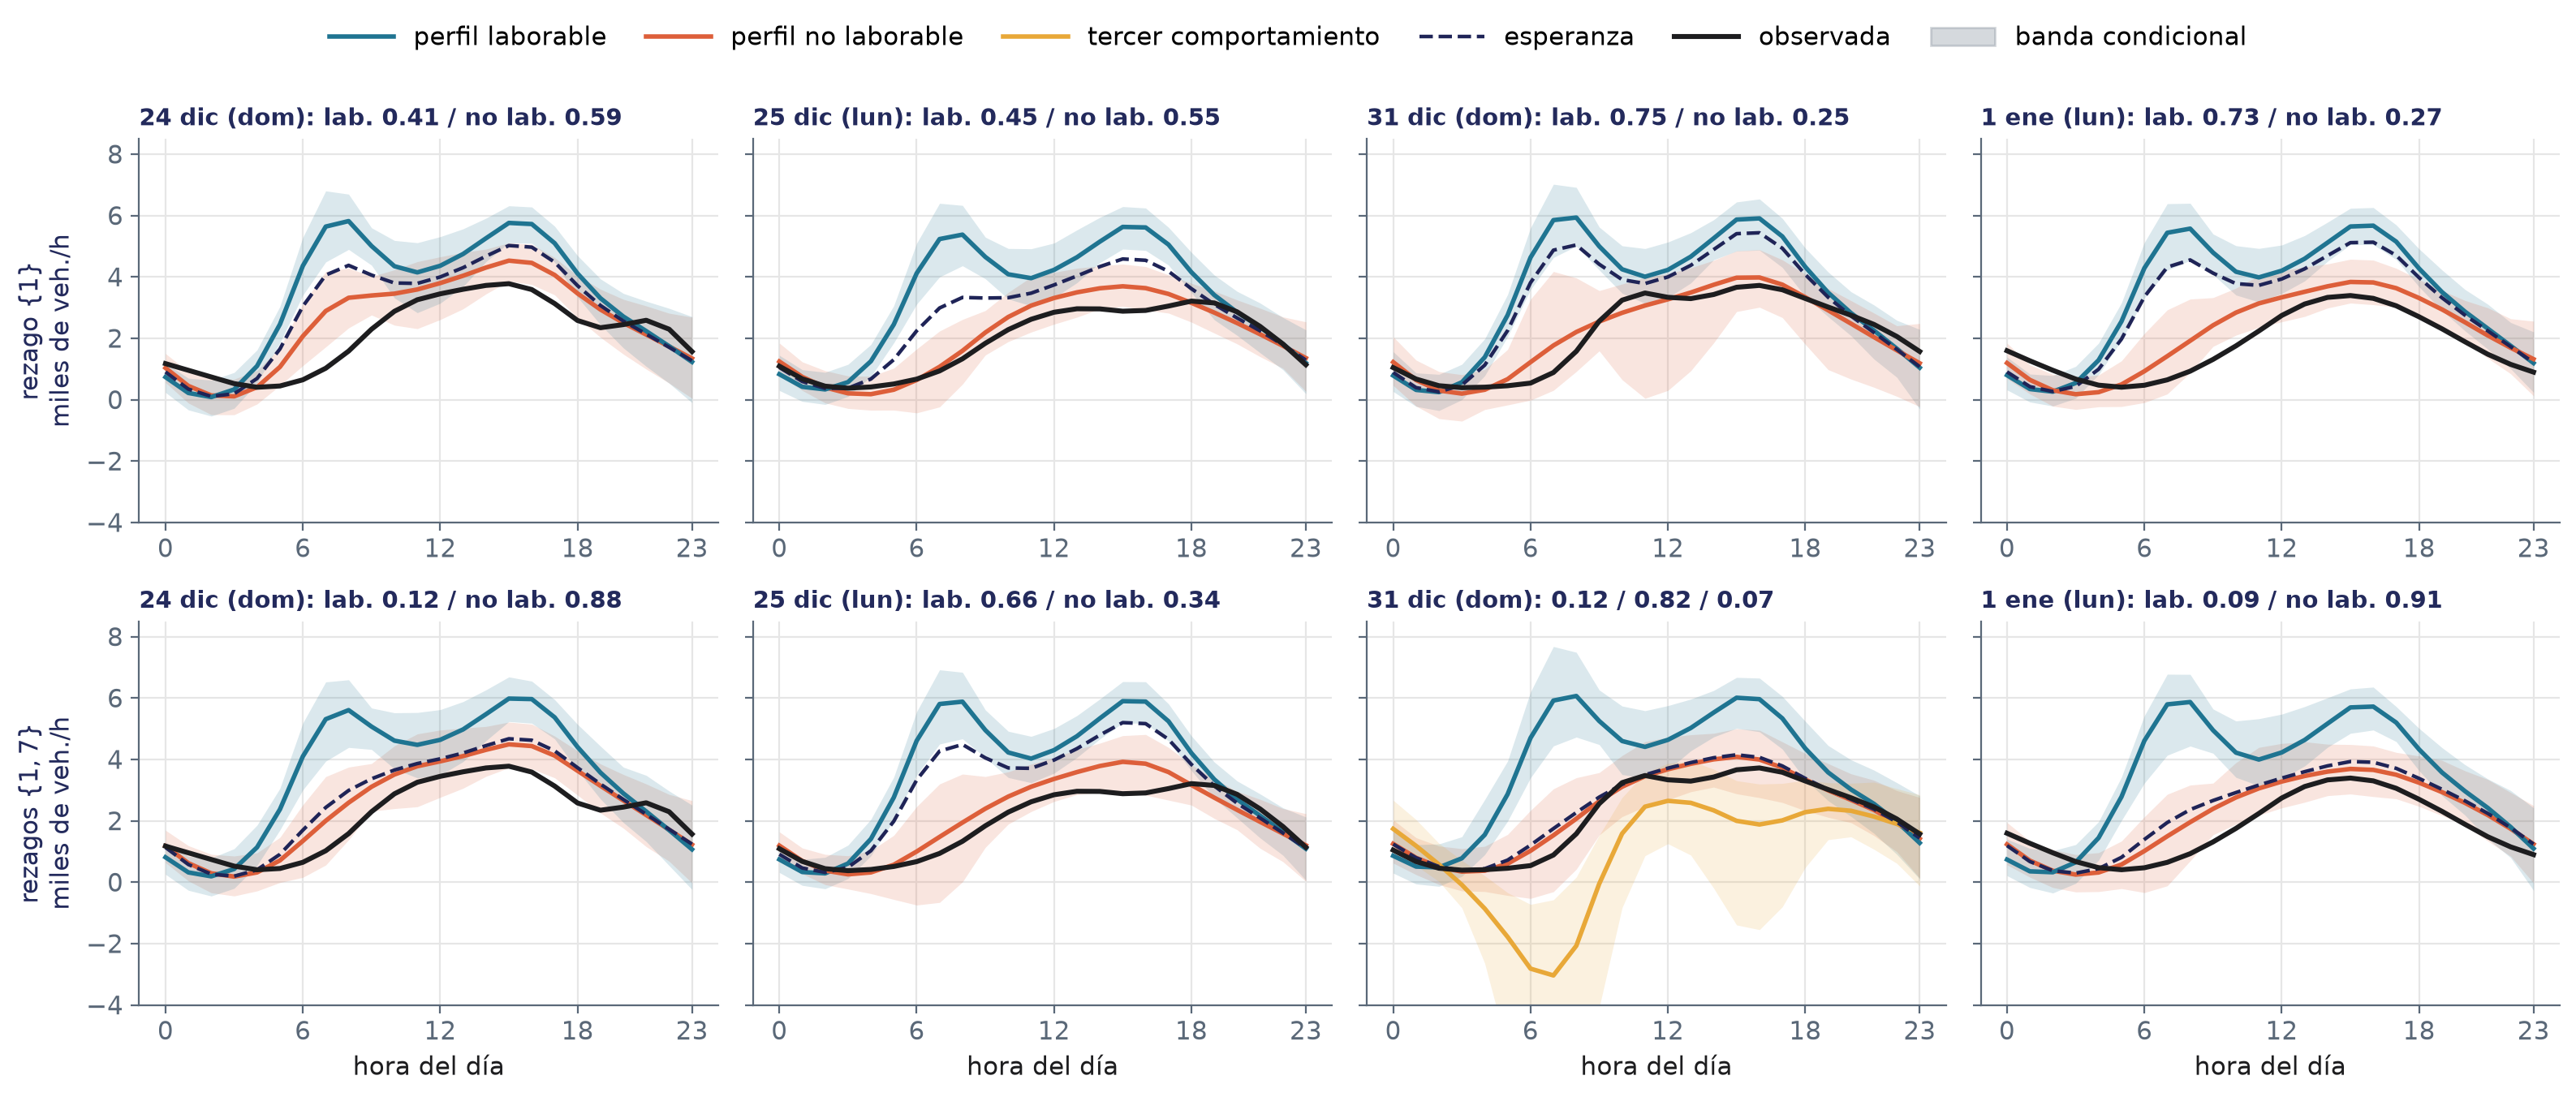
\includegraphics[width=\textwidth]{IMG/04_03/04_ventana_detalle.png}
\caption{Cuatro orígenes de la ventana de detalle, con rezago $\{1\}$ (arriba) y rezagos $\{1,7\}$ (abajo) ($M = 10$): curva observada, esperanza y, por comportamiento, curva típica y banda condicional. Los comportamientos se nombran por su perfil y el título da la probabilidad de cada uno; con tres comportamientos, en orden de nivel.}
\label{fig:apl_ventana_detalle}
\end{figure}

La Figura~\ref{fig:apl_ventana_detalle} muestra cuatro días de la ventana de detalle. En los orígenes con dos comportamientos, uno tiene la forma del día laborable, con sus dos horas punta, y el otro la del fin de semana, con un solo máximo al mediodía, y la esperanza queda entre ambos, en una curva con horas punta atenuadas que no corresponde a ningún día. Con el rezago de un día, el 24 y el 25 de diciembre el comportamiento más probable es el no laborable y la curva observada lo sigue, aunque con probabilidades cercanas a un medio. El 31 de diciembre y el 1 de enero el más probable es el laborable y la curva observada sigue al comportamiento minoritario, que el modelo mantiene con una probabilidad cercana a un cuarto y cuya banda la contiene, lo que corresponde al caso en que una predictiva con más de un comportamiento ofrece una opción que el promedio no tiene.\\

Con ambos rezagos la masa se desplaza hacia el perfil correcto, de modo que el no laborable recibe $0.88$ el 24 de diciembre, $0.82$ el 31 y $0.91$ el 1 de enero, porque el lunes anterior fue Navidad y el rezago semanal anuncia el feriado. La excepción es la propia Navidad, un lunes precedido por un lunes laborable, en que el rezago semanal empuja la masa hacia el perfil laborable ($0.66$) y la curva observada sigue al minoritario. La información del rezago semanal resuelve el tipo de día cuando la semana anterior lo anuncia, y no cuando no lo anuncia. Los diez orígenes de la ventana se muestran en el Anexo~\ref{aneC_00_00_trafico}.\\

Los comportamientos funcionan, por tanto, como un agrupamiento de la curva siguiente por tipo de día, el estado latente que el calendario registra y que no entra al modelo. Para medirlo, en cada origen con dos comportamientos se identifica el de perfil no laborable como el de menor nivel medio y se lo cruza con el día predicho (Cuadro~\ref{tab:apl_K_tipo}).

% Fuente: comportamientos_psbp.npz de 101 y 102 (test, K = 2) y 65_comportamientos_calendario.csv; el perfil
% no laborable es el comportamiento de menor nivel medio; "observada más cerca" = menor distancia L2 a la curva típica.
\begin{table}[H]
\centering\small
\setlength{\tabcolsep}{4pt}
\caption{Comportamientos y tipo de día en los orígenes de prueba con dos comportamientos ($M = 10$). Fracción en que el comportamiento más probable corresponde al tipo de día predicho, probabilidad media de ese comportamiento y fracción en que la curva observada queda más cerca de él que del otro.}
\label{tab:apl_K_tipo}
\begin{tabular}{l l c ccc}
\hline
Rezagos & Día predicho & Orígenes & Más probable & Probabilidad & Observada \\
 & & & corresponde & media & más cerca \\
\hline
$\{1\}$   & Laborable    & 155 & 95.5\% & 0.80 & 96.8\% \\
          & No laborable & 101 & 55.4\% & 0.55 & 96.0\% \\
          & Todos        & 256 & 79.7\% & 0.70 & 96.5\% \\
\hline
$\{1,7\}$ & Laborable    & 35  & 65.7\% & 0.63 & 94.3\% \\
          & No laborable & 90  & 95.6\% & 0.83 & 97.8\% \\
          & Todos        & 125 & 87.2\% & 0.77 & 96.8\% \\
\hline
\end{tabular}
\end{table}

En las dos especificaciones la curva observada queda más cerca del comportamiento que corresponde a su tipo de día en el $96\%$ a $97\%$ de los orígenes, de modo que los dos comportamientos corresponden a los dos tipos de día. Lo que cambia con la información no es el agrupamiento sino la probabilidad que recibe cada grupo. Con el rezago de un día el modelo acierta el tipo de los días laborables, porque la mayoría siguen a otro laborable, pero en los no laborables el comportamiento correcto es el más probable solo en el $55\%$ de los casos, cerca de lo que daría el azar. Con el rezago semanal ese acierto sube al $96\%$, con una probabilidad media de $0.83$. Los pocos laborables que conservan dos comportamientos son sobre todo lunes (20 de 35), en que el rezago de un día viene de un fin de semana, y en ellos el acierto baja al $66\%$.

\subsection{Predicción por comportamiento}
\label{04_03_04_pronostico}

Los Cuadros~\ref{tab:apl_pronostico_101} y~\ref{tab:apl_pronostico_102} resumen el error del pronóstico por comportamiento y de su cota frente a la esperanza y a las referencias, sobre todos los orígenes de prueba y sobre los que tienen más de un comportamiento. Como en la simulación, se promedia sobre los orígenes y no sobre las ventanas, porque el subconjunto con más de un comportamiento no es contiguo, y por eso las cifras difieren en la tercera decimal de las del error puntual.

% Fuente: 113_opciones_por_origen.csv (m10, test, opción "tipica") y 119_resumen_opciones_por_M.csv;
% MAE = media por origen, RMSE = raíz de la media de cuadrados por origen.
\begin{table}[H]
\centering\small
\setlength{\tabcolsep}{4pt}
\caption{Pronóstico por comportamiento en el bloque de prueba del tráfico con rezago $\{1\}$ ($M = 10$), sobre todos los orígenes y sobre los que tienen más de un comportamiento.}
\label{tab:apl_pronostico_101}
\begin{tabular}{l cc cc}
\hline
& \multicolumn{2}{c}{Todos ($n = 357$)} & \multicolumn{2}{c}{$K_t \ge 2$ ($n = 256$)} \\
 & MAE & RMSE & MAE & RMSE \\
\hline
Pronóstico por comportamiento & 0.386 & 0.719 & 0.417 & 0.779 \\
Cota (mejor comportamiento) & 0.269 & 0.432 & 0.254 & 0.382 \\
Esperanza & 0.409 & 0.650 & 0.449 & 0.688 \\
FAR & 0.390 & 0.620 & 0.431 & 0.654 \\
Random Forest & 0.357 & 0.568 & 0.384 & 0.590 \\
\hline
El pronóstico gana al FAR & \multicolumn{2}{c}{56\%} & \multicolumn{2}{c}{66\%} \\
El pronóstico gana al Random Forest & \multicolumn{2}{c}{51\%} & \multicolumn{2}{c}{58\%} \\
La cota gana al FAR & \multicolumn{2}{c}{70\%} & \multicolumn{2}{c}{85\%} \\
La cota gana al Random Forest & \multicolumn{2}{c}{64\%} & \multicolumn{2}{c}{75\%} \\
Acierto (el mejor es el más probable) & \multicolumn{2}{c}{85\%} & \multicolumn{2}{c}{79\%} \\
\hline
\end{tabular}
\end{table}

\begin{table}[H]
\centering\small
\setlength{\tabcolsep}{4pt}
\caption{Pronóstico por comportamiento en el bloque de prueba del tráfico con rezagos $\{1,7\}$ ($M = 10$), sobre todos los orígenes y sobre los que tienen más de un comportamiento.}
\label{tab:apl_pronostico_102}
\begin{tabular}{l cc cc}
\hline
& \multicolumn{2}{c}{Todos ($n = 357$)} & \multicolumn{2}{c}{$K_t \ge 2$ ($n = 128$)} \\
 & MAE & RMSE & MAE & RMSE \\
\hline
Pronóstico por comportamiento & 0.300 & 0.550 & 0.413 & 0.718 \\
Cota (mejor comportamiento) & 0.259 & 0.435 & 0.299 & 0.445 \\
Esperanza & 0.306 & 0.528 & 0.431 & 0.669 \\
FAR & 0.306 & 0.499 & 0.380 & 0.587 \\
Random Forest & 0.307 & 0.504 & 0.410 & 0.619 \\
\hline
El pronóstico gana al FAR & \multicolumn{2}{c}{61\%} & \multicolumn{2}{c}{56\%} \\
El pronóstico gana al Random Forest & \multicolumn{2}{c}{63\%} & \multicolumn{2}{c}{66\%} \\
La cota gana al FAR & \multicolumn{2}{c}{65\%} & \multicolumn{2}{c}{66\%} \\
La cota gana al Random Forest & \multicolumn{2}{c}{68\%} & \multicolumn{2}{c}{79\%} \\
Acierto (el mejor es el más probable) & \multicolumn{2}{c}{95\%} & \multicolumn{2}{c}{86\%} \\
\hline
\end{tabular}
\end{table}

El pronóstico por comportamiento elige, como en la simulación, uno de los perfiles posibles, y eso tiene un costo cuando elige mal. Con el rezago de un día baja el MAE de la esperanza en un $6\%$ sobre todos los orígenes y en un $7\%$ sobre los que tienen más de un comportamiento, queda al nivel del FAR y supera al FAR y al Random Forest en la mayoría de los orígenes con más de un comportamiento, pero es peor en RMSE que todas las alternativas, porque cuando acierta, su error es menor que el de la esperanza, y cuando elige el perfil incorrecto, el error es el de un día laborable predicho como fin de semana, o al revés, y el promedio cuadrático lo penaliza. Con ambos rezagos la mayoría de los orígenes tiene un solo comportamiento, el pronóstico coincide con la esperanza en ellos y sobre todos los orígenes es el mejor en MAE ($0.300$); en los orígenes que conservan más de un comportamiento, que son sobre todo fines de semana y feriados, el FAR queda por debajo.\\

La cota indica cuánto se puede ganar al elegir bien. Con el rezago de un día, en los orígenes con más de un comportamiento, la cota baja el MAE de la esperanza en un $43\%$ y queda bajo el Random Forest en tres de cada cuatro orígenes, de modo que entre las opciones que entrega el modelo casi siempre está la buena, y la pérdida se produce al elegirla según la probabilidad. Con ambos rezagos la distancia entre el pronóstico y la cota se reduce, porque la información que antes repartía la masa entre dos opciones ahora decide por una de ellas.

% Fuente: 115_ventana_modelos_w30.csv del _06 de 101 y 102 (test, opción "tipica").
\begin{figure}[H]
\centering
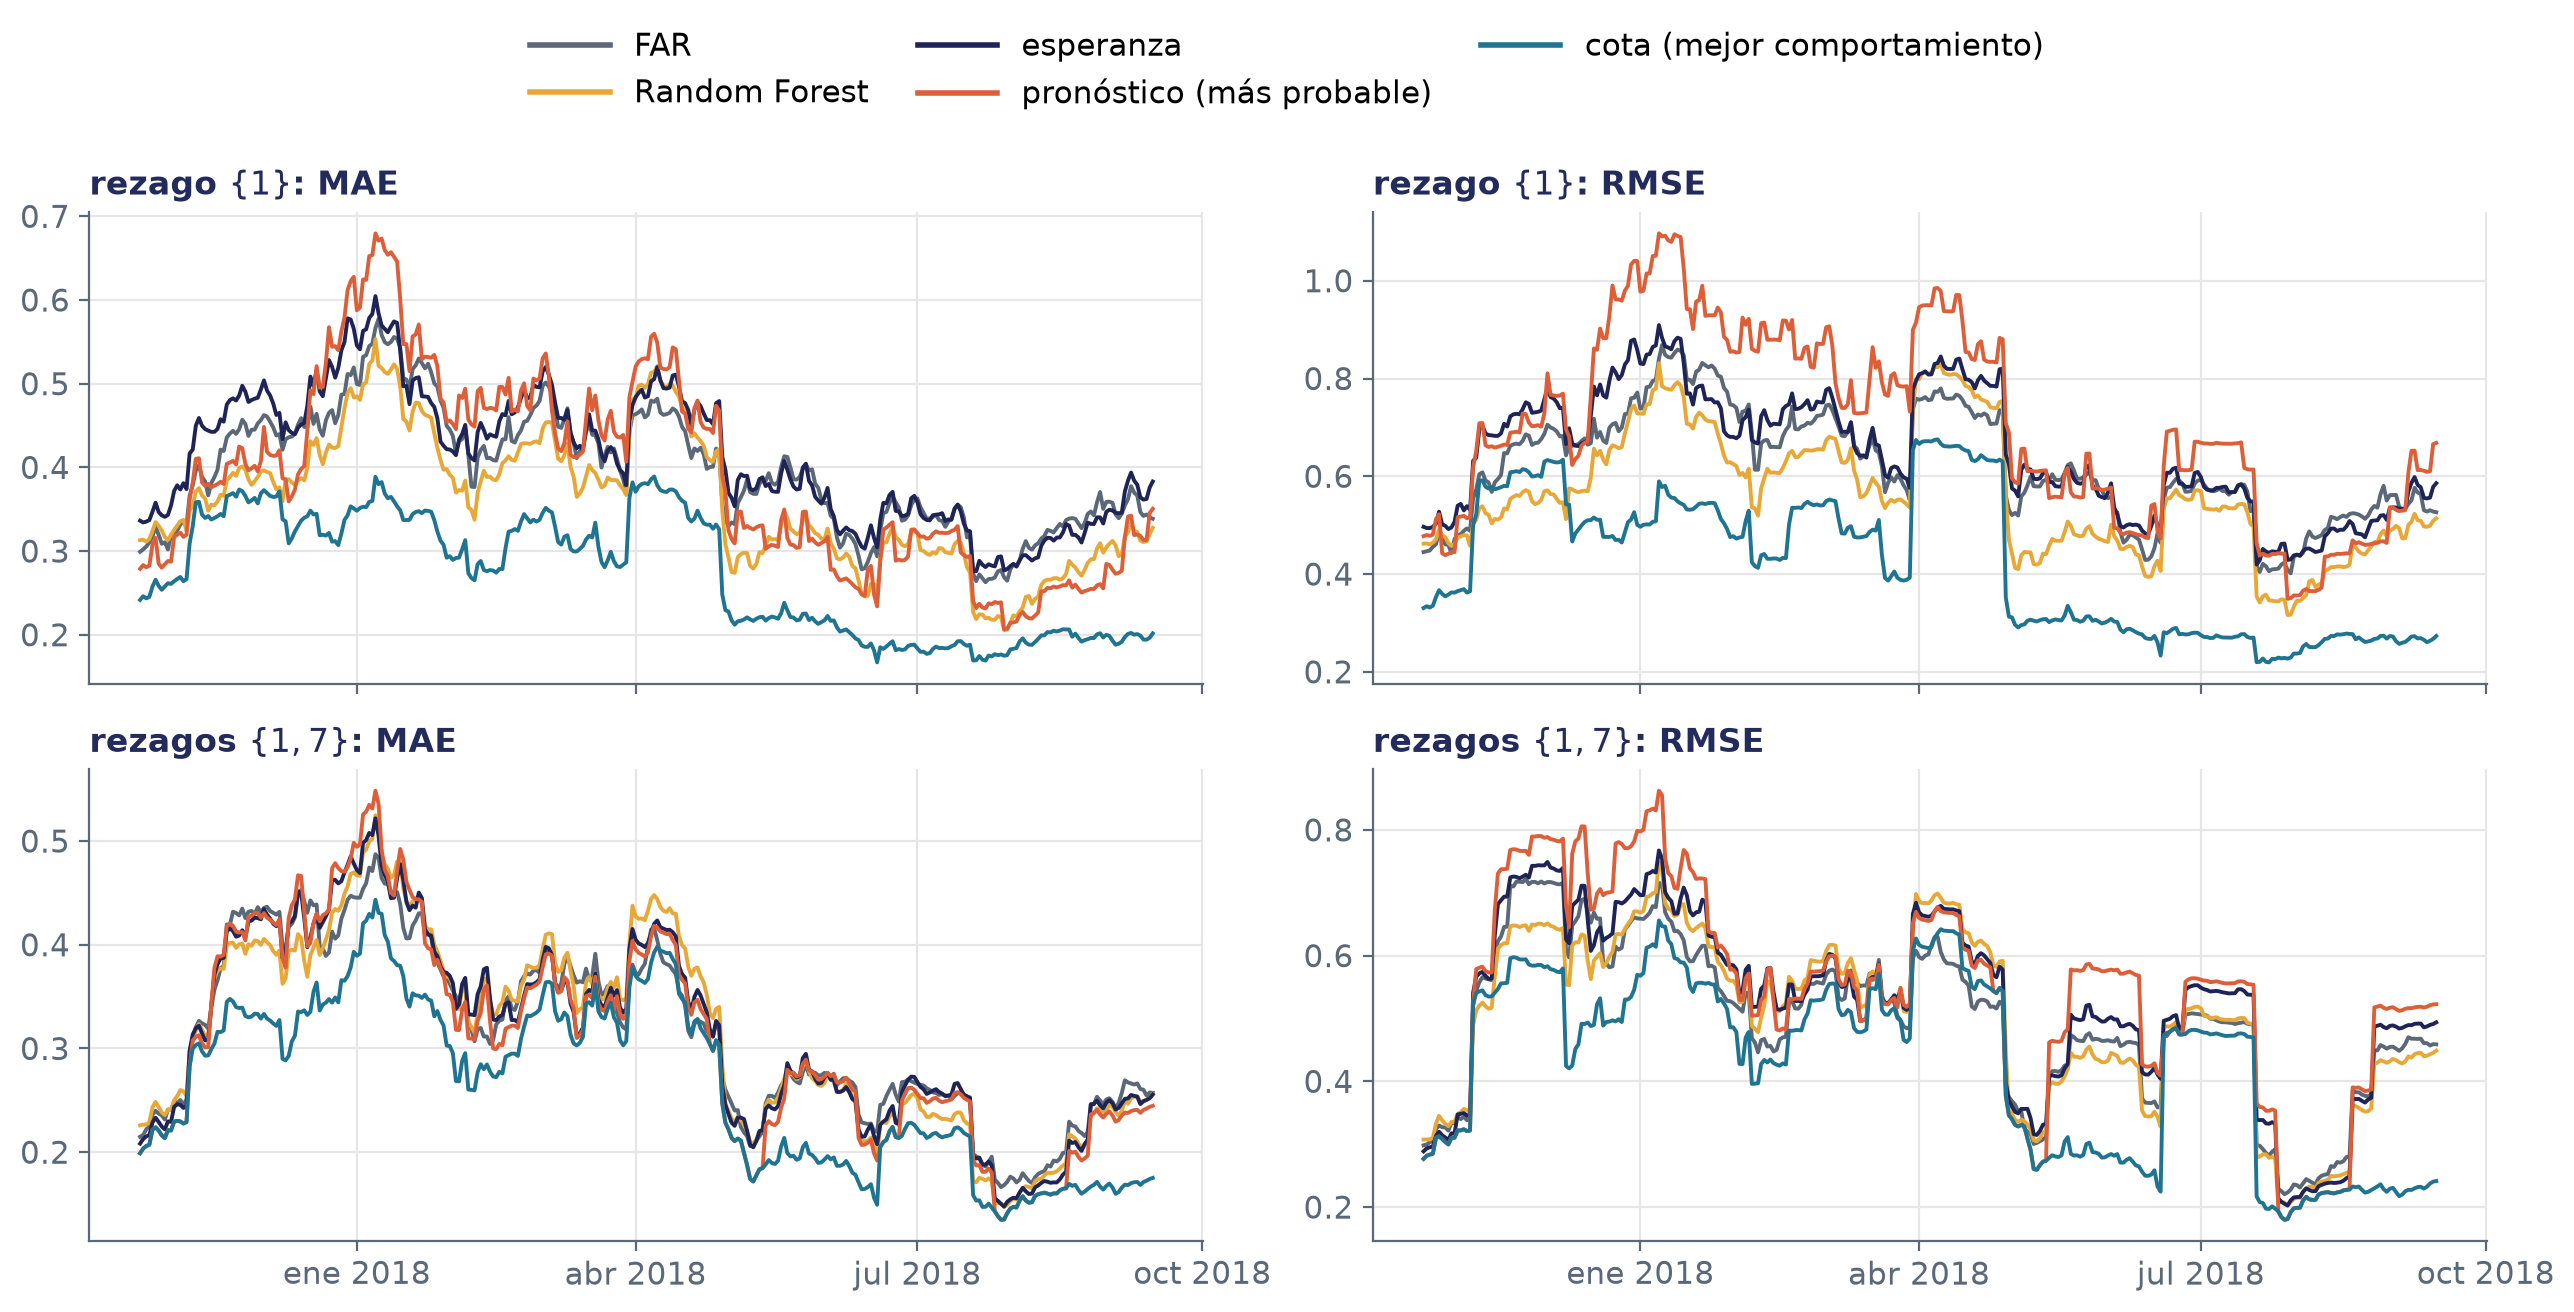
\includegraphics[width=\textwidth]{IMG/04_03/04_pronostico_ventana_w30.png}
\caption{MAE y RMSE del pronóstico por comportamiento y de la cota sobre la ventana móvil del bloque de prueba, junto a la esperanza, el FAR y el Random Forest, con rezago $\{1\}$ (arriba) y rezagos $\{1,7\}$ (abajo) ($M = 10$, $w = 30$).}
\label{fig:apl_pronostico_ventana}
\end{figure}

La Figura~\ref{fig:apl_pronostico_ventana} muestra lo mismo a lo largo del bloque de prueba. Con el rezago de un día la cota queda bajo todos los modelos en todas las ventanas, y el pronóstico se separa hacia arriba en RMSE entre diciembre y mayo, donde elegir el perfil incorrecto tiene más costo. Con ambos rezagos el pronóstico y la esperanza casi coinciden, y la cota se separa de ellos solo en algunos tramos, que son los que conservan más días con dos comportamientos.

% Fuente: 119_acierto_por_p1.csv (test, K >= 2, M = 10).
\begin{table}[H]
\centering\small
\setlength{\tabcolsep}{3.5pt}
\caption{Acierto del pronóstico por comportamiento ($K_t \ge 2$, $M = 10$) por tramo de la probabilidad del comportamiento elegido y MAE que se pierde por no elegir el mejor, en promedio sobre los orígenes del tramo.}
\label{tab:apl_acierto_p1}
\begin{tabular}{l ccc ccc}
\hline
 & \multicolumn{3}{c}{Rezago $\{1\}$} & \multicolumn{3}{c}{Rezagos $\{1,7\}$} \\
$p_{t,k^{*}}$ & Orígenes & Acierto & Pérdida & Orígenes & Acierto & Pérdida \\
\hline
$[0.5, 0.6)$ & 38 & 47\% & 0.45 & 3 & 67\% & 0.18 \\
$[0.6, 0.7)$ & 41 & 66\% & 0.24 & 9 & 78\% & 0.27 \\
$[0.7, 0.8)$ & 59 & 75\% & 0.20 & 22 & 64\% & 0.22 \\
$[0.8, 0.9)$ & 71 & 93\% & 0.04 & 52 & 88\% & 0.11 \\
$[0.9, 1]$ & 47 & 98\% & 0.01 & 42 & 98\% & 0.03 \\
\hline
\end{tabular}
\end{table}

El Cuadro~\ref{tab:apl_acierto_p1} muestra que, con el rezago de un día, el acierto sube de forma monótona con la probabilidad, de un $47\%$ entre $0.5$ y $0.6$, donde elegir equivale al azar, a un $98\%$ sobre $0.9$, y la pérdida respecto de la cota cae de $0.45$ a $0.01$. Con ambos rezagos la masa se desplaza hacia las probabilidades altas, porque la información decide el perfil. La lectura práctica es la misma que en la simulación, con una probabilidad alta se pronostica con el comportamiento más probable y con una baja se reportan las opciones y sus probabilidades.

\subsection{Selección de variables}
\label{04_03_05_seleccion}

El mecanismo de inclusión de la ecuación~\eqref{eq:gamma_prior} permite identificar qué scores rezagados afectan la ley del score que se modela. Para cada score respuesta $\xi_{tm}$ y cada covariable se reporta la probabilidad posterior de inclusión (PIP), la probabilidad de que la covariable entre en al menos uno de los átomos ocupados de la mezcla de ese score, estimada como la frecuencia de ese evento en las iteraciones retenidas. Una PIP cercana a uno indica que el rezago correspondiente interviene en la mezcla del score, y una cercana a cero, que la mezcla prescinde de él.

% Fuente: osumout y N1out de las trazas chain_fpc_<k>_iter01.mat de 101 y 102, burn = 1000; coincide con 46_pip.csv del _03.
\begin{figure}[H]
\centering
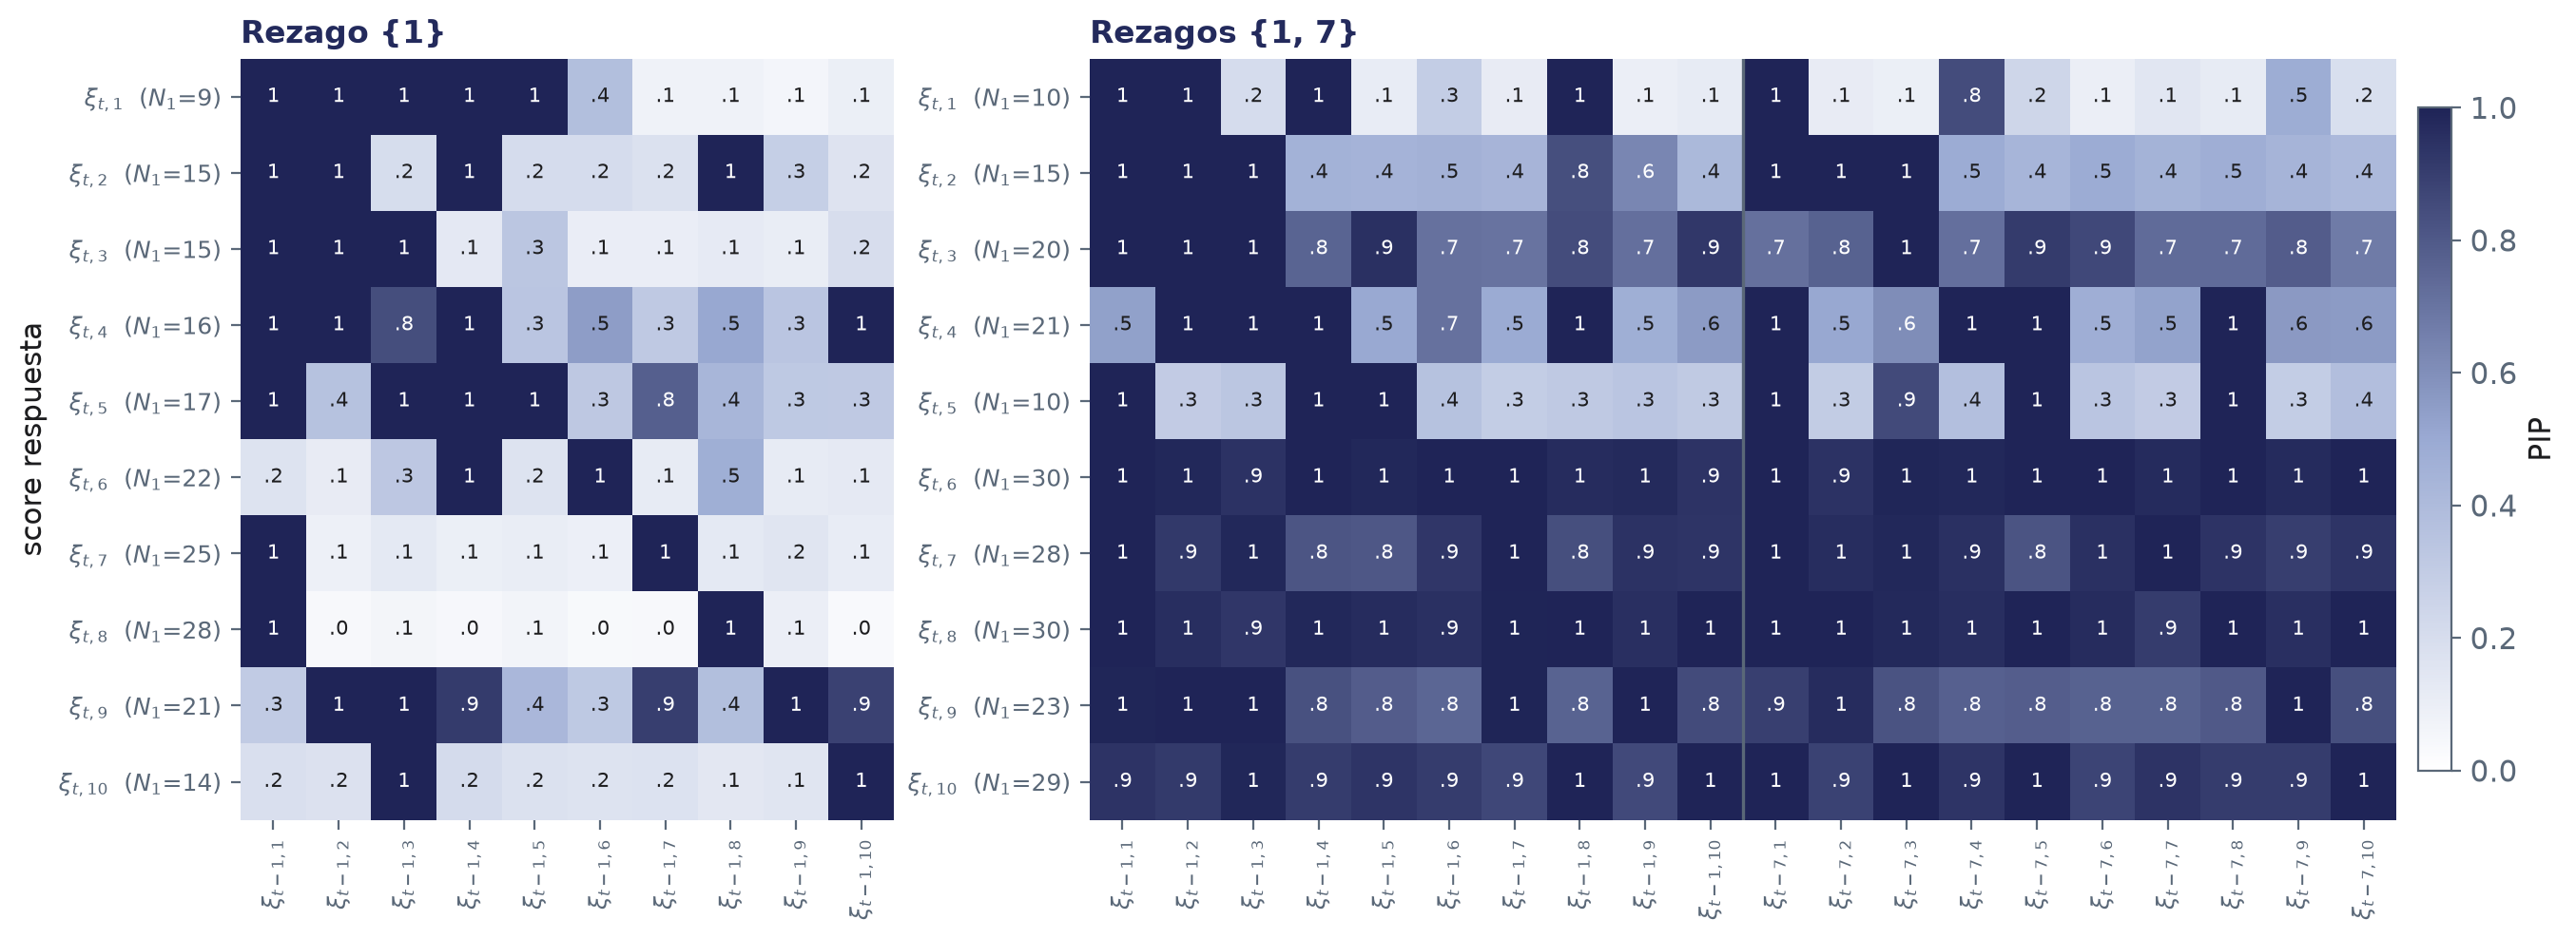
\includegraphics[width=\textwidth]{IMG/04_03/04_pip.png}
\caption{Probabilidad posterior de inclusión de cada covariable (columnas) en la mezcla de cada score (filas), con rezago $\{1\}$ (izquierda) y rezagos $\{1,7\}$ (derecha) ($M = 10$). $\xi_{t-\ell,m}$ es el score $m$ del día $t-\ell$, y $N_1$, el índice medio del último átomo ocupado de la mezcla, sobre un truncamiento de 30.}
\label{fig:apl_pip}
\end{figure}

La Figura~\ref{fig:apl_pip} muestra que, con el rezago de un día, la mezcla del primer score incluye los rezagos de los cinco primeros scores con PIP igual a uno y excluye los otros cinco, con PIP de $0.38$ o menos; la del segundo incluye los scores $1$, $2$, $4$ y $8$, y la del tercero los tres primeros. Todos los scores incluyen su propio rezago, y el rezago del primer score entra en siete de las diez mezclas.\\

Con el rezago semanal, la mezcla del primer score conserva del día anterior los scores $1$, $2$, $4$ y $8$, excluye los scores $3$ y $5$, y de la semana anterior incluye solo el primer score, con PIP igual a uno, y el cuarto, con $0.85$; los otros ocho rezagos semanales quedan en $0.48$ o menos. La mezcla del segundo score agrega los rezagos semanales de los tres primeros scores, y la del quinto los de los scores $1$, $3$, $5$ y $8$. El rezago semanal del primer score entra con PIP igual a uno en las mezclas de los scores $1$, $2$, $4$ y $5$.\\

En las mezclas que ocupan casi todo el truncamiento, la PIP no distingue entre covariables. Con el rezago semanal, las mezclas del tercer score y de los scores $6$ a $10$ ocupan entre 20 y 30 átomos, y en ellas todas las covariables tienen PIP de $0.67$ o más. Como la PIP cuenta la inclusión en cualquier átomo ocupado, es posible que con tantos átomos se acerque a uno sin que todas las covariables sean relevantes. El detalle de estas mezclas está en el Anexo~\ref{aneC_00_09_seleccion}. Con una sola cadena por especificación, además, la PIP no tiene una medida de su variabilidad entre cadenas y se lee como descriptiva.
\section{Discusión}
\label{04_04_00_discusion}

La aplicación al tráfico confirma en datos reales lo que el estudio de simulación mostraba en el escenario C-2. Cuando la ley de la curva siguiente depende de un estado que las covariables solo revelan en parte, la predictiva del PSBPM-FD reparte su masa entre comportamientos que corresponden a estados reconocibles del proceso, aquí el perfil laborable y el de fin de semana, y esa estructura se traduce en intervalos mejores que los de un modelo lineal con banda de ancho fijo, con un Winkler un $11\%$ menor que el del FAR en ambas especificaciones y menor en el $93\%$ de las ventanas con el rezago de un día y en el $76\%$ con ambos rezagos. En el error puntual la ventaja depende del resumen. Bajo MAE la mediana puntual supera al FAR en un $5.4\%$ con el rezago de un día y en un $3.7\%$ con ambos rezagos, y le gana en el $70\%$ y el $80\%$ de las ventanas, respectivamente; con ambos rezagos es además el mejor predictor en MAE y el que gana más ventanas, un $59\%$. Bajo RMSE, en cambio, la esperanza no supera al FAR, y el Random Forest es el mejor predictor puntual cuando solo se dispone del día anterior.\\

La comparación entre las dos especificaciones muestra el efecto de la información sobre los pesos de la mezcla. Al agregar el rezago semanal, la mezcla concentra la masa en un solo comportamiento en los días en que esa información decide el perfil, de martes a viernes, y conserva varios comportamientos donde no lo decide, en fines de semana, feriados y lunes. El modelo no impone la multimodalidad, más bien la produce cuando la información disponible no basta para elegir entre estados. Los comportamientos funcionan además como un agrupamiento por tipo de día, el estado latente que no entra al modelo, ya que la curva observada queda cerca del comportamiento de su tipo de día en el $96\%$ de los orígenes con dos comportamientos, y lo que la información cambia es la probabilidad que recibe cada grupo, que en los días no laborables pasa de acertar el perfil en algo más de la mitad de los casos a acertarlo en casi todos. Esa misma información mejora a todos los métodos y elimina las diferencias entre ellos en el error puntual, pero no en los intervalos, donde el PSBPM-FD mantiene su ventaja porque su ancho sigue al estado del proceso.\\

Estos resultados descansan en supuestos estructurales del modelo. La factorización de la ecuación~\eqref{eq:factorizacion} modela cada score con una mezcla univariada y supone independencia condicional entre componentes, un supuesto más razonable para los scores de la FPCA, que no están correlacionados, que para los coeficientes de una base fija, que en general lo están. Por eso el modelo trabaja sobre los scores y no directamente sobre los coeficientes, aun cuando la base sea ortonormal. Además, para que el modelo sea competitivo es necesario retener prácticamente tantos scores como coeficientes de la base, aquí $M = J = 10$, de modo que la representación conserva los detalles de la curva y no solo una versión suavizada de ella.\\

Esa misma elección condiciona la interpretación de la selección de variables. Las autofunciones de la FPCA se extienden sobre todo el dominio, de modo que un score no corresponde a un intervalo particular de $\tau$, y la PIP indica qué scores rezagados afectan a cada score sin traducirse directamente en qué horas del día anterior afectan a qué horas del día siguiente. Obtener esa interpretación requeriría una base local que conserve la estructura de cada tramo del dominio, como las B-splines, pero sus coeficientes están correlacionados, y al tratarse de mezclas univariadas y no de un modelo para el vector completo no pueden usarse directamente sin contradecir el supuesto de la factorización. La interpretabilidad de la selección y la factorización por componentes quedan así en tensión.\\

Por último, las otras cinco series del Anexo~\ref{aneD_00_00_otras_series}, sin un estado oculto que separe perfiles, tienen predictivas unimodales, y en ellas el PSBPM-FD queda cerca del FAR, lo que delimita el alcance de la ventaja que muestra el tráfico a series cuya ley condicional tiene más de un comportamiento.